\section{Background estimation}
\label{sec:htoinv_background_estimation}

Accurate estimation of the \acrlong{sm} background processes in the signal region is paramount to a search for new physics. Mismeasured backgrounds and uncertainties can wash out traces of signal and affect the fit to data. To aid in this endeavour, several regions of phase space aside from the signal region are explored in the analysis. The \glspl{CR} and \glspl{SB} aid in the prediction of the \acrshort{sm} electroweak and \acrshort{qcd} multijet backgrounds, respectively. They are separated by \acrlong{hlt} requirements, and object selections in the \glspl{CR} or kinematic selections in the \glspl{SB}.

The single lepton \glspl{CR} are used to constrain, specifically, the lost lepton background in the signal region, arising primarily from \ttbarpjets and \wtolnupjets as a missed lepton would serve as a source of \ptvecmiss. The dilepton and photon \glspl{CR} predict the \ztonunu background. The former parallels the decay as it is enriched in \ztolplmpjets---possessing the same kinematic properties while being much easier to detect, improving statistical accuracy. The latter region substitutes the \ztonunu decay with a photon, permissible as long as the momentum of the photon is large compared to the \PZ mass. 

These estimations rely on the distributions of data and \acrlong{mc} in those regions, controlled via rate parameters to connect them to the signal region. \Glspl{SB} to the signal region estimate \acrshort{qcd} multijet contributions from data. The prediction in this case takes the form of a \emph{transfer factor} method---a constrained application of a rate parameter. Prediction of the background yields from each of these methods is done so within the fit and expressed in the likelihood functions. Further explanation of the mechanics is given in the remainder of this section. Fig.~\ref{fig:htoinv_fit_overview} illustrates the correspondence between the analysis regions and background predictions.

\begin{figure}[htbp]
    \centering
    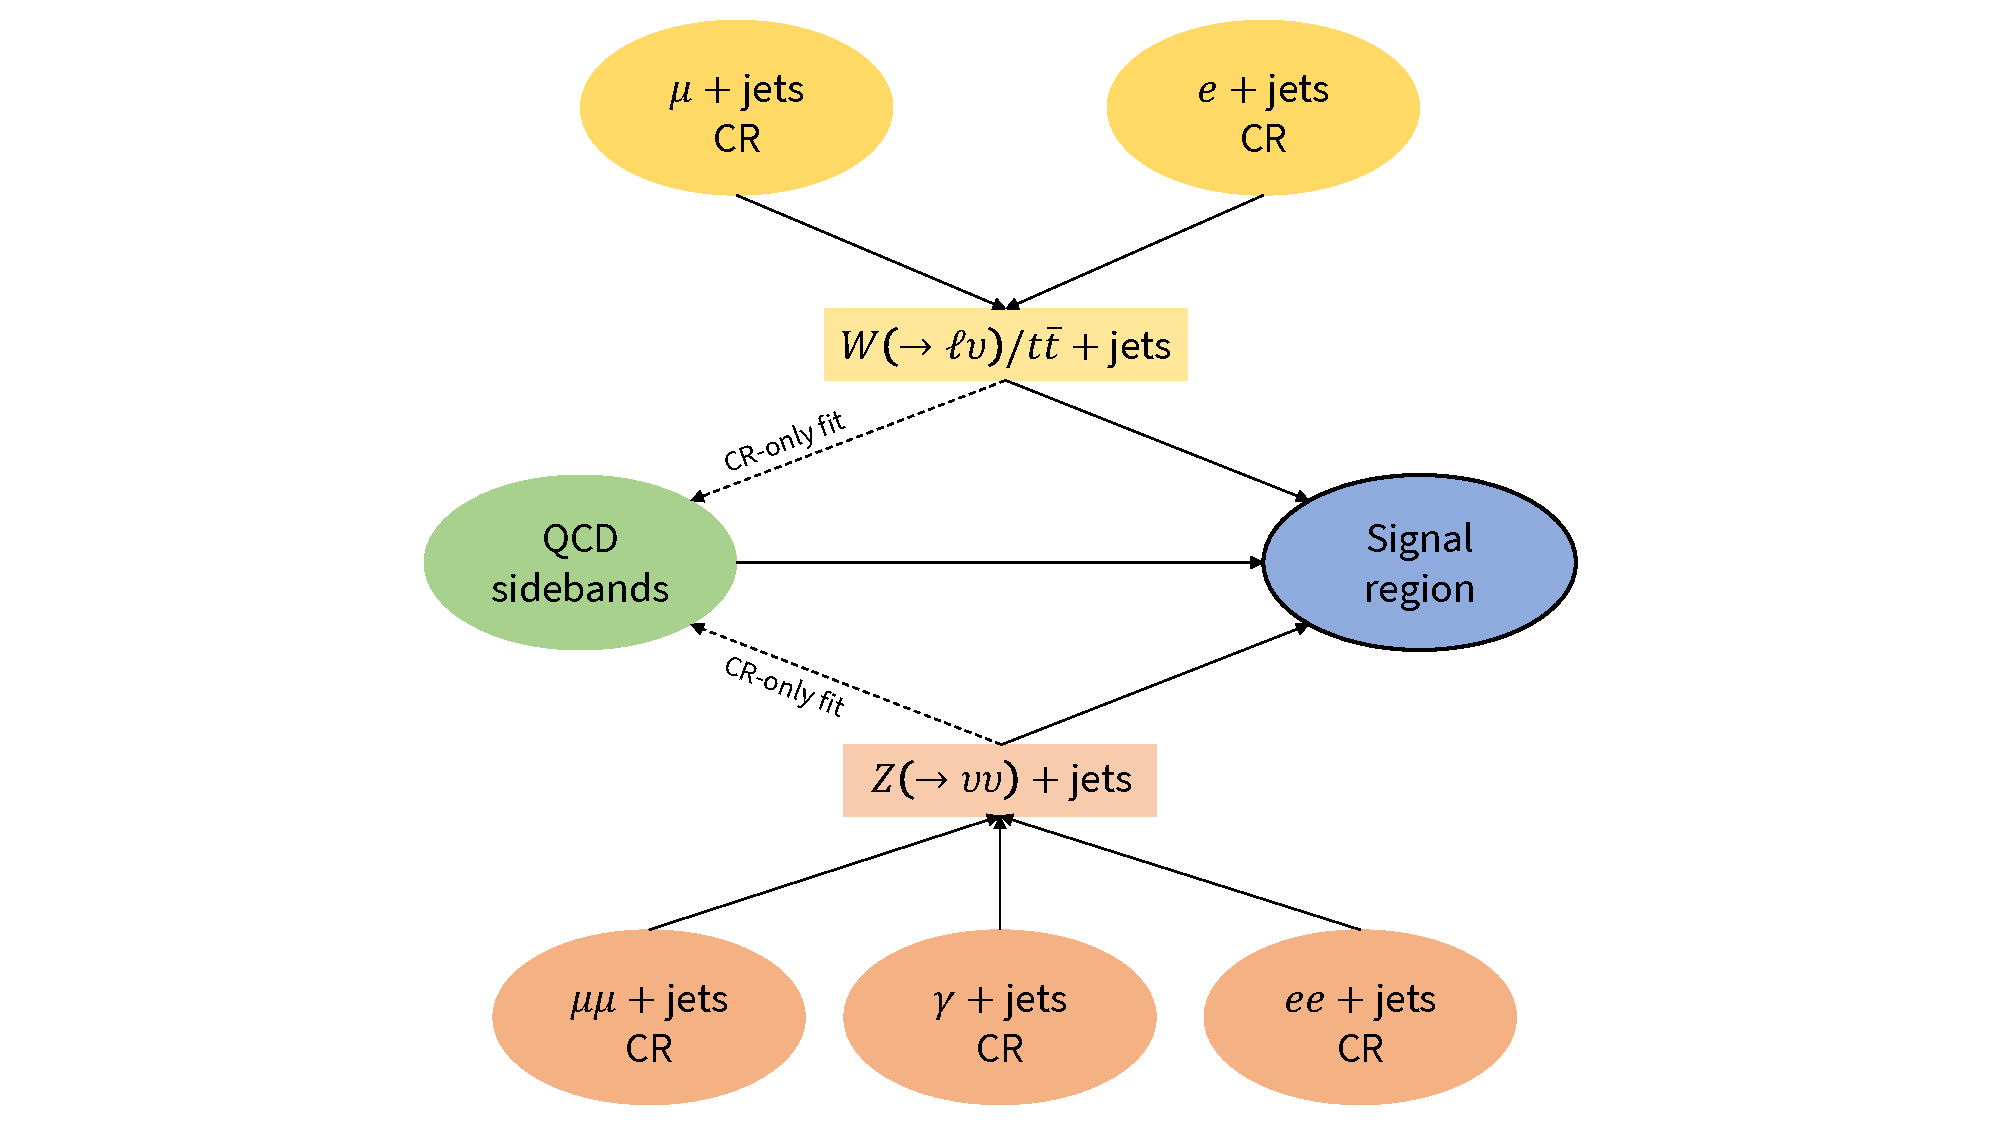
\includegraphics[width=0.5\textwidth]{figures/fit_overview.pdf}
    \caption[An infographic showcasing the role of each analysis region in the fit to data]{An infographic showcasing the role of each analysis region in the fit to data. The \glspl{CR} predict the lost lepton and \ztonunu backgrounds, and a \gls{CR}-only fit informs the \acrshort{qcd} multijet prediction that contributes to the eventual background determination in the signal region.}
    \label{fig:htoinv_fit_overview}
\end{figure}


%=========================================================


\subsection{Control regions}
\label{subsec:htoinv_control_regions}

\Glspl{CR} serve two complementary purposes in many analyses: the prediction of certain backgrounds that dominate in the signal region, as a more accurate method than using the yields directly from \acrlong{mc}; and to validate the data, \acrshort{mc}, and corrections applied. They are orthogonal to the signal region and to each other by way of lepton or photon requirements, and by triggers that may pertain to those objects. \Glspl{CR} are designed to, ideally, be devoid of signal given their role as \acrshort{sm} descriptors. Contamination is sometimes present, but at a very small level. Five \glspl{CR} are used in the analysis: \singleMuCr, \doubleMuCr, \singleEleCr, \doubleEleCr, and \singlePhotonCr. The criteria for the objects---which are defined explicitly in Chpt.~\ref{sec:analysis_objects}---are summarised in the list below:
\medskip
\begin{easylist}[itemize]
    \easylistprops
    & \singleMuCr: one tight muon \tightMuon with $\pt > \text{20}\GeV$ and a transverse mass (as calculated in Eq.~\ref{eq:transverse_mass_massless}) in the range $\text{50} < \mtMuon < \text{110}\GeV$
    & \doubleMuCr: one tight muon \tightMuon with $\pt > \text{20}\GeV$, and one loose muon \looseMuon with $\pt > \text{10}\GeV$ that has opposite charge, with a combined invariant mass of $\text{60} < \doubleMuMass < \text{120}\GeV$ in the \VH categories, while instead $\text{75} < \doubleMuMass < \text{105}\GeV$ in the \ttH categories. The leading muon is required to possess $\pt > \text{110}\GeV$
    & \singleEleCr: one tight electron \tightEle with $\pt > \text{40}\GeV$ and $\text{50} < \mtElectron < \text{110}\GeV$
    & \doubleEleCr: one tight electron \tightEle with $\pt > \text{40}\GeV$, and one veto electron \vetoEle with $\pt > \text{10}\GeV$ that has opposite charge, with a combined invariant mass of $\text{60} < \doubleEleMass < \text{120}\GeV$ in the \VH categories, while instead $\text{75} < \doubleEleMass < \text{105}\GeV$ in the \ttH categories. The leading electron is required to possess $\pt > \text{110}\GeV$
    & \singlePhotonCr: one medium photon \mediumPhoton with $\pt > \text{230}\GeV$
\end{easylist}

\medskip

\noindent{}The event selection for the \glspl{CR} mirrors the signal region almost exactly, with few exceptions that are detailed in Chpt.~\ref{subsec:htoinv_other_filters}. The only other differentiation is the \acrshort{qcd} suppression criteria from Tab.~\ref{tab:htoinv_categories}. These are applied in the signal region, but not to any of the \glspl{CR} for the \ttH categories. This was to improve the statistical accuracy in the \glspl{CR}, notably in the otherwise depleted dilepton regions, and was found to avoid compromising the data--simulation agreement and the shapes of the important distributions. For the \VH categories, the \acrshort{qcd} suppression criteria were included in the \glspl{CR} as the shape of the \ptmiss distribution was found to be different depending on whether the criteria were included or not. The \glspl{CR} in those categories were also not deficient in events, unlike in the case of \ttH.

The transverse mass cuts in the single lepton \glspl{CR} reduce the effect of signal contamination, specifically from \ttH since its \mT generally eclipses that of \ttbar.\footnote{The \mT for a \ttbar event with \ptvecmiss solely from the neutrino (in $\HepProcess{\Ptop \to \Pbottom\PW}$, $\HepProcess{\PW \to \Plepton\Pnu}$) should be in a window around the \PW mass. Introducing additional decay products such as the Higgs boson increase it.} The trigger requirements for the \singleMuCr and \doubleMuCr \glspl{CR} are the same as for the signal region (Tab.~\ref{tab:htoinv_SR_triggers}) since the same \gls{PD} is used.

In the \doubleMuCr and \doubleEleCr \glspl{CR}, the \doubleLepMass window is halved for the \ttH categories compared to the others to reduce contamination from dileptonic \ttbar decays, granting a a higher purity \ztolplmpjets region. The leading lepton \pt requirement is increased in these regions for all categories, also for purity purposes.

The \singleEleCr and \doubleEleCr \glspl{CR} take advantage of the increased statistical power of two \glspl{PD} in both 2016 and 2017, characterised by electron and photon triggers. In 2018, they were merged into a single $\Pe/\Pphoton$ \gls{PD}. Tabs.~\ref{tab:htoinv_ele_pd_triggers} and~\ref{tab:htoinv_photon_pd_triggers} elucidate how the trigger requirements are specified for each year. As before, each quantity and object is defined at \acrshort{hlt} level. If an event aims to enter the \singleEleCr or \doubleEleCr, and is from the dataset of \Pe-based triggers, the criteria for either of the two triggers for the given year in Tab.~\ref{tab:htoinv_ele_pd_triggers} must be satisfied. If an event aims to enter either \gls{CR} and is from the \gls{PD} of \Pphoton-based triggers, the failure of both of the electron triggers in Tab.~\ref{tab:htoinv_ele_pd_triggers} and the passing of any of the photon triggers in Tab.~\ref{tab:htoinv_photon_pd_triggers} are required. This condition avoids double counting events that also appear in the electron trigger-based dataset. In 2018, any of the year's triggers in Tabs.~\ref{tab:htoinv_ele_pd_triggers} and~\ref{tab:htoinv_photon_pd_triggers} may be satisfied since there is only one \gls{PD}. For \acrlong{mc} events, as the datasets are not categorised by trigger, they may pass any of the requirements for their respective year in either table.

\begin{table}[htbp]
    \centering
    \begin{tabular}{ccccc}
        \toprule
        Year & $E_{\mathrm{T}, \,\mathrm{SC}}^{\Pe}$ threshold (\GeVns) & \Pe WP & Calorimeter ID & \acrshort{gsf} track-SC matching \\ \midrule
        \multirow{2}{*}{2016} & 27 & Tight & --- & --- \\
        & 105 & --- & Very tight & Tight \\
        \midrule
        \multirow{2}{*}{2017} & 35 & Tight & --- & --- \\
        & 115 & --- & Very tight & Tight \\
        \midrule
        \multirow{2}{*}{2018} & 32 & Tight & --- & --- \\
        & 115 & --- & Very tight & Tight \\
        \bottomrule
    \end{tabular}
    \caption[The trigger requirements for events to enter the \singleEleCr or \doubleEleCr control regions, if they originate from the dataset of \Pe-based triggers]{The trigger requirements for events to enter the \singleEleCr or \doubleEleCr \glspl{CR}, if they originate from the dataset of \Pe-based triggers. Selections are on the transverse energy of the supercluster $E_{\mathrm{T}, \,\mathrm{SC}}$, the working point of the candidate electron, ID of the candidate in the calorimeters, and the matching between the \acrfull{gsf}-fitted track and supercluster, all at \acrshort{hlt} level.}
    \label{tab:htoinv_ele_pd_triggers}
\end{table}

\begin{table}[htbp]
    \centering
    \begin{tabular}{ccc}
        \toprule
        Year & $\ET^{\Pphoton}$ threshold (\GeVns) & $H/E$ \\\midrule
        \multirow{2}{*}{2016} & 165 & $< \text{0.1}$ \\
        & 175 & --- \\
        \midrule
        2017 & 200 & --- \\
        \midrule
        2018 & 200 & --- \\
        \bottomrule
    \end{tabular}
    \caption[The trigger requirements for events to enter the \singleEleCr \doubleEleCr, or \singlePhotonCr control regions, if they originate from the dataset of \Pphoton-based triggers]{The trigger requirements for events to enter the \singleEleCr \doubleEleCr, or \singlePhotonCr \gls{CR}, if they originate from the dataset of \Pphoton-based triggers. Selections are on the transverse energy \ET of the candidate, and the ratio of the candidate's central energy deposit in the \acrshort{hcal} to the \acrshort{ecal} ($H/E$), all computed at \acrshort{hlt} level.}
    \label{tab:htoinv_photon_pd_triggers}
\end{table}

For the \singlePhotonCr \gls{CR}, data is used from \acrshort{cms} originating only from the dataset of \Pphoton-based triggers. Data and \acrshort{mc} must satisfy any of the triggers from Tab.~\ref{tab:htoinv_photon_pd_triggers} for the respective year.

In each of the \glspl{CR}, the \ptvecmiss is recalculated without the objects used to define said region as a proxy for \ptvecmiss in the signal region. Conditions in the event selection and binning that refer to \ptvecmiss or \ptmiss use this recalculated quantity when applied to the \glspl{CR}. Using the \singleMuCr \gls{CR} as an example, the new \ptvecmiss is the vector sum of the old \ptvecmiss and the tight muon's \ptvec.

The relative composition of the background processes in each \gls{CR} after the analysis-level selection is summarised in Fig.~\ref{fig:htoinv_cr_composition_comb2016to18}. As desired, the single lepton \glspl{CR} are very similar and dominated by the \ttbar and \wtolnu processes. The dilepton regions also possess a very similar composition to each other, enriched in Drell-Yan \ztoll, and to a lesser extent \ttbar and $\ttbar X$ which contain several dileptonic decay channels.  In the \singlePhotonCr \gls{CR}, expectedly the \gammapjets process dominates virtually every category. \acrshort{qcd} multijet events make up a consistent, small fraction of the events. Rather than the yields from \acrshort{mc} as they would likely consist of \glspl{jet} misidentified as photons, its presence in this region is estimated from a data driven purity measurement explained in Chpt.~\ref{subsubsec:htoinv_photon_purity}.

\begin{figure}[htbp]
    \centering
    \begin{subfigure}[b]{0.33\textwidth}
        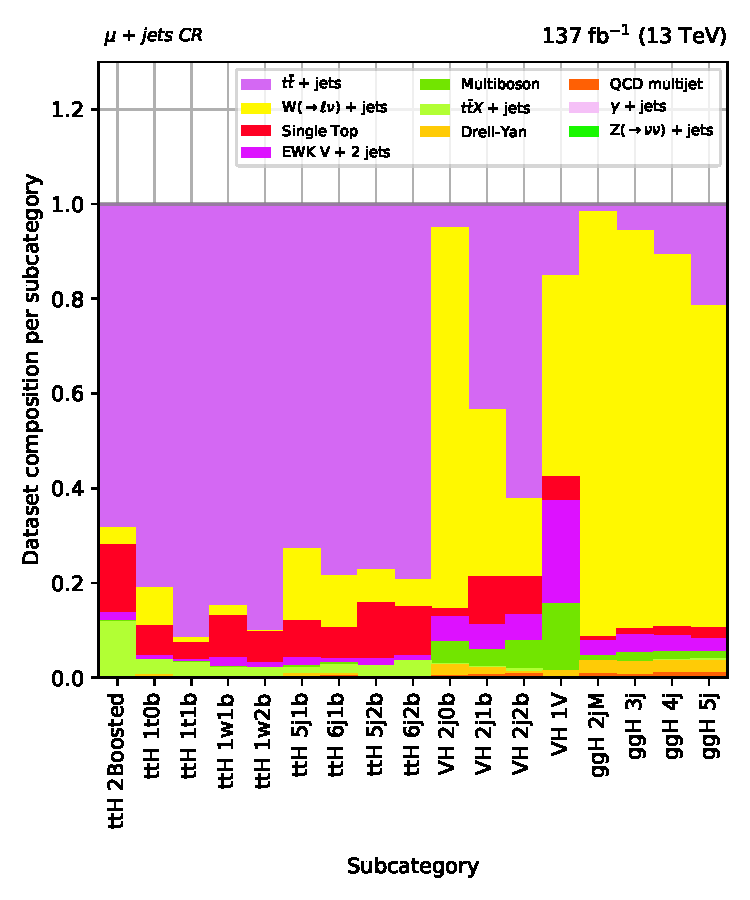
\includegraphics[width=\textwidth]{figures/region_plots/full_Run2/region_1/background_composition.pdf}
        \caption{\singleMuCr control region}
    \end{subfigure}
    \hspace{0.05\textwidth}
    \begin{subfigure}[b]{0.33\textwidth}
        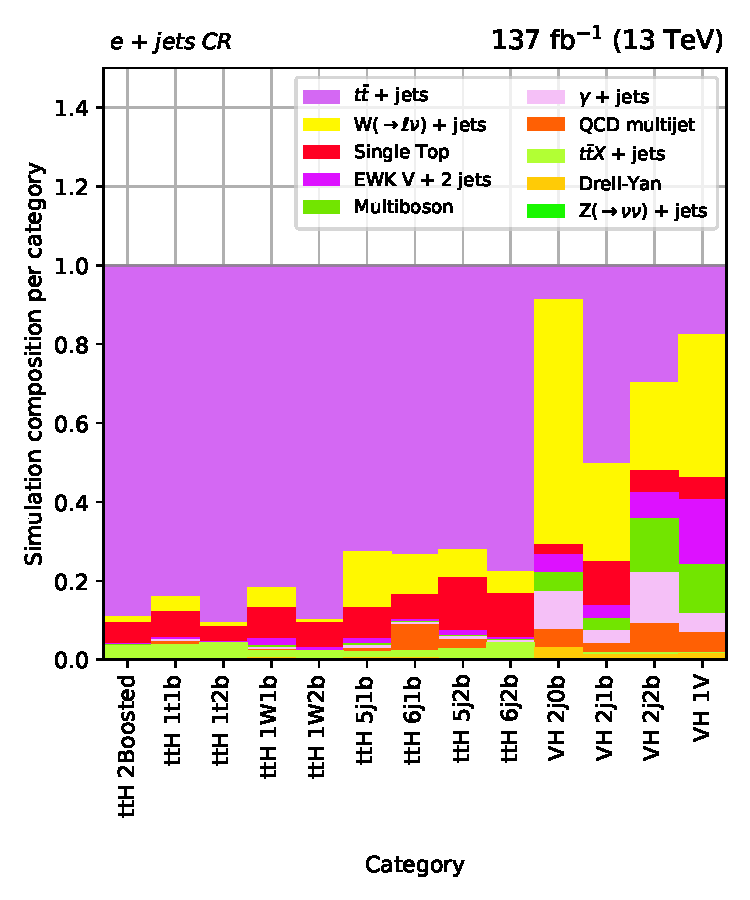
\includegraphics[width=\textwidth]{figures/region_plots/full_Run2/region_3/background_composition.pdf}
        \caption{\singleEleCr control region}
    \end{subfigure}

    \begin{subfigure}[b]{0.33\textwidth}
        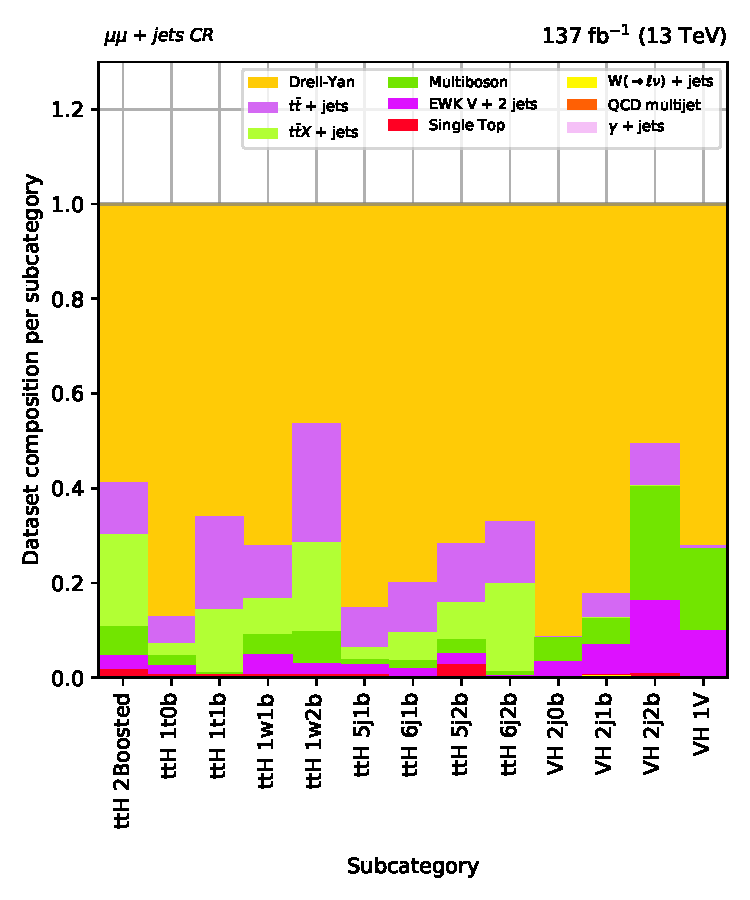
\includegraphics[width=\textwidth]{figures/region_plots/full_Run2/region_2/background_composition.pdf}
        \caption{\doubleMuCr control region}
    \end{subfigure}
    \hspace{0.05\textwidth}
    \begin{subfigure}[b]{0.33\textwidth}
        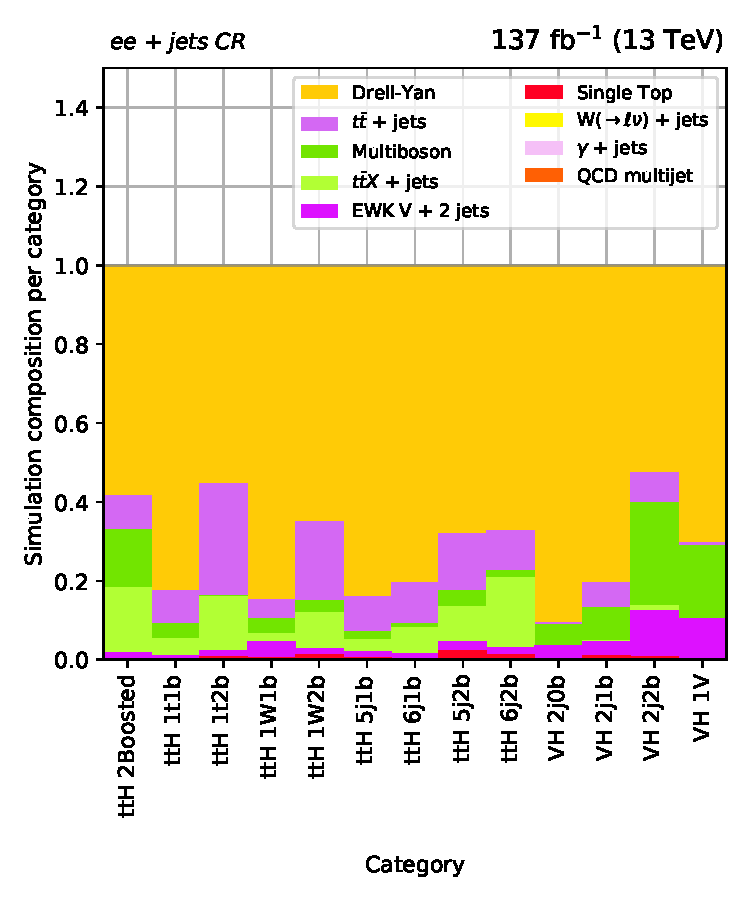
\includegraphics[width=\textwidth]{figures/region_plots/full_Run2/region_4/background_composition.pdf}
        \caption{\doubleEleCr control region}
    \end{subfigure}

    \begin{subfigure}[b]{0.33\textwidth}
        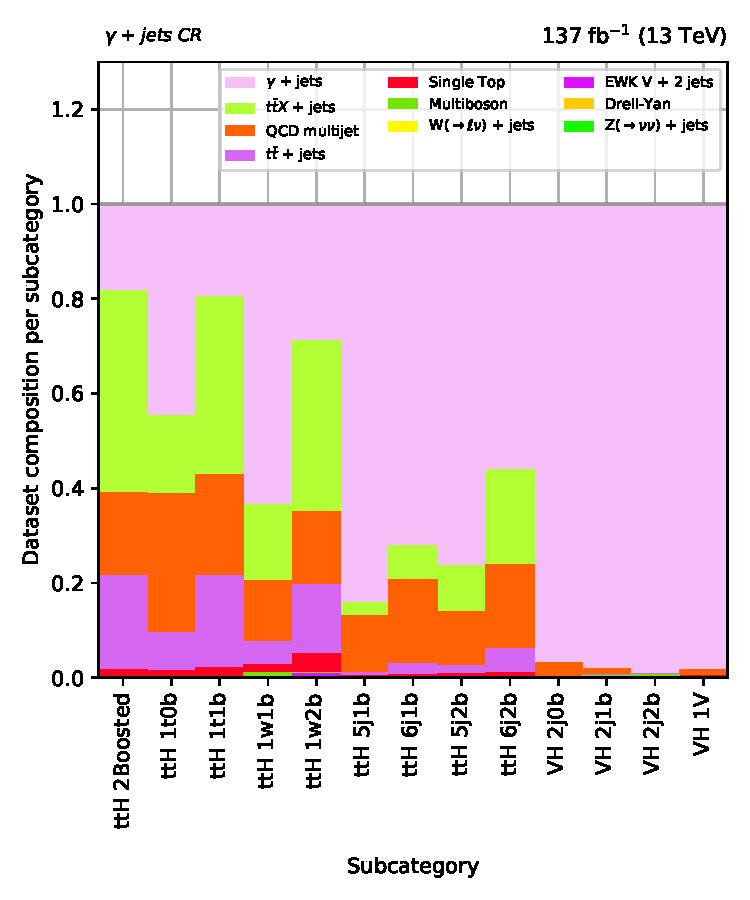
\includegraphics[width=\textwidth]{figures/region_plots/full_Run2/region_5/background_composition.pdf}
        \caption{\singlePhotonCr control region}
    \end{subfigure}
    \caption[Composition of each category in each of the control regions for simulated background processes after the analysis-level selection]{Composition of each category in each of the control regions for simulated background processes after the analysis-level selection.}
    \label{fig:htoinv_cr_composition_comb2016to18}
\end{figure}


%=========================================================


\subsection{Lost lepton background estimation}
\label{subsubsec:htoinv_lost_lepton_bkg}

In order to predict the lost lepton background in the signal region, a freely floating rate parameter $a_{\lostlepton}$ is introduced in the fit. It is shared across the single lepton \glspl{CR} and signal region, where it scales the event count from simulation in these regions to obtain the expected values. Events are categorised and binned in the same manner in the single lepton \glspl{CR} as in the signal region, such that the rate parameters---and therefore the prediction---is derived bin-by-bin. The predicted number of lost lepton events in Eqs.~\ref{eq:likelihood_SR} and \ref{eq:likelihood_CRs} is then simply $b_{\lostlepton} \cdot a_{\lostlepton}$.

Distributions of the single lepton \glspl{CR} after the \gls{CR}-only fit are illustrated in Figs.~\ref{fig:htoinv_mountain_range_2017_single_lep_ttH} and \ref{fig:htoinv_mountain_range_2017_single_lep_VH} in the \ttH and \VH categories, respectively, for the 2017 dataset. Corresponding event counts, along with the rate parameters, can be found in Tab.~\ref{tab:htoinv_rate_params_2017_lost_lep}. Equivalent figures for the other data taking periods are accessible in Apps.~\ref{sec:pre_post_fit_plots_ttH_CRs} and \ref{sec:pre_post_fit_plots_VH_CRs} for the \ttH and \VH categories, respectively.

\clearpage

\begin{figure}[htbp]
    \centering
    \begin{subfigure}[b]{\textwidth}
        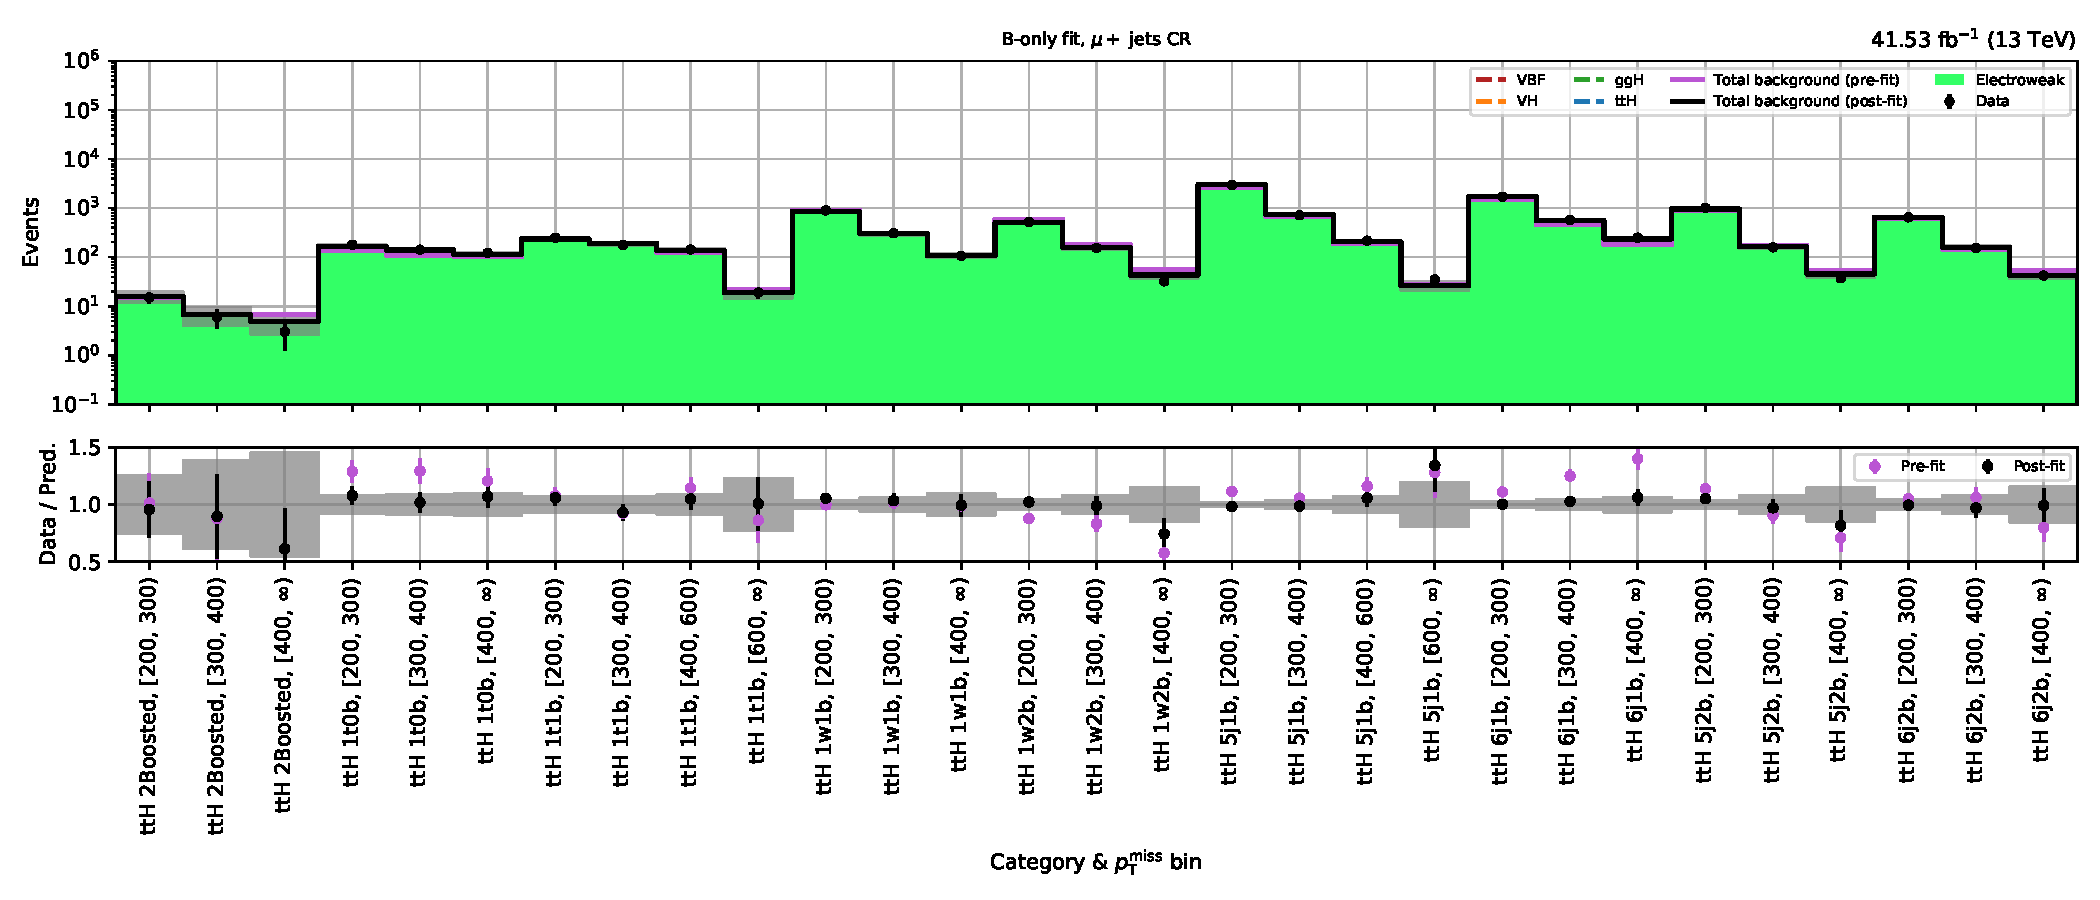
\includegraphics[width=\textwidth]{chapters/higgstoinv/figures/mountain_ranges/2017/ttH/Wmunu_tree_fit_b-abs_values_ttH_cats.pdf}
        \caption{\ttH --- \singleMuCr \gls{CR} (2017)}
    \end{subfigure}

    \begin{subfigure}[b]{\textwidth}
        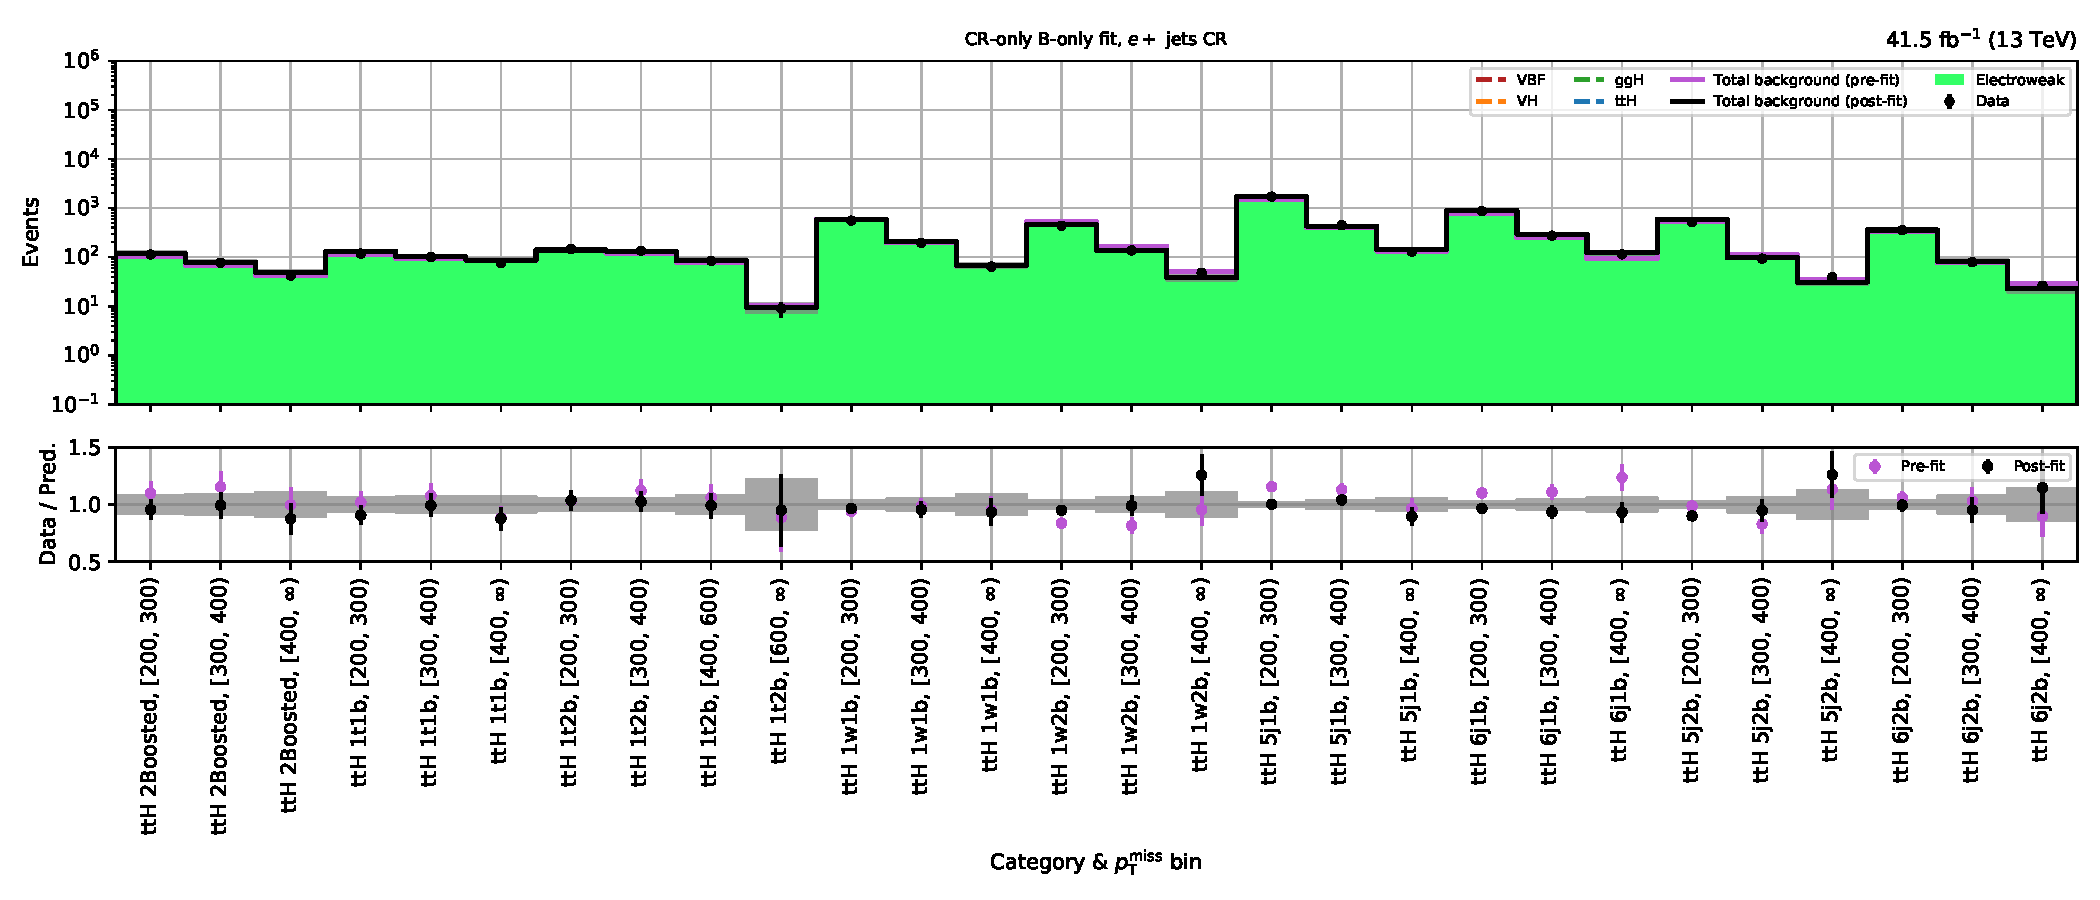
\includegraphics[width=\textwidth]{chapters/higgstoinv/figures/mountain_ranges/2017/ttH/Wenu_tree_fit_b-abs_values_ttH_cats.pdf}
        \caption{\ttH --- \singleEleCr \gls{CR} (2017)}
    \end{subfigure}
    \caption[Post-fit yields for each category and \ptmiss bin in the single lepton control regions of the \ttH categories for the 2017 dataset]{Post-fit yields for each category and \ptmiss bin in the single lepton \glspl{CR} of the \ttH categories for the 2017 dataset. The total background pre-fit and post-fit is compared to data in the lower panel of each subfigure.}
    \label{fig:htoinv_mountain_range_2017_single_lep_ttH}
\end{figure}

\begin{figure}[htbp]
    \centering
    \begin{subfigure}[b]{\textwidth}
        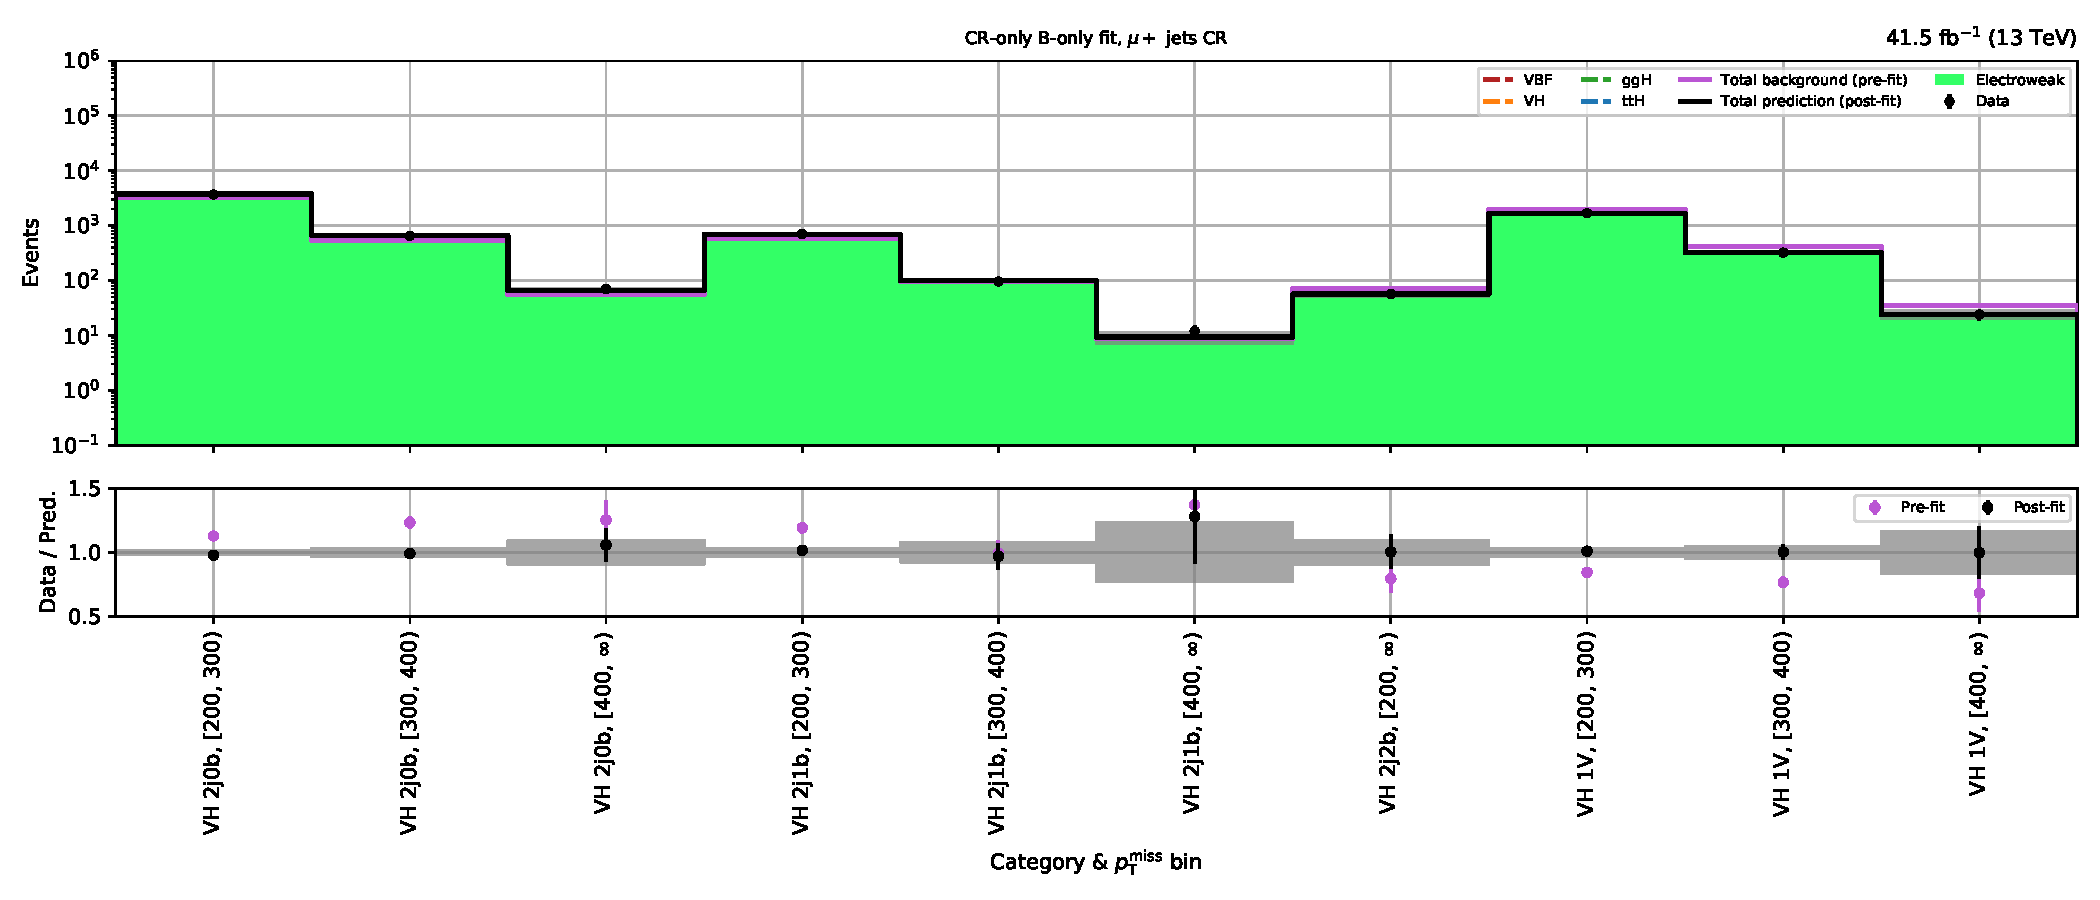
\includegraphics[width=\textwidth]{chapters/higgstoinv/figures/mountain_ranges/2017/VH/Wmunu_tree_fit_b-abs_values_VH_cats.pdf}
        \caption{\VH --- \singleMuCr \gls{CR} (2017)}
    \end{subfigure}
    \hfill
    \begin{subfigure}[b]{\textwidth}
        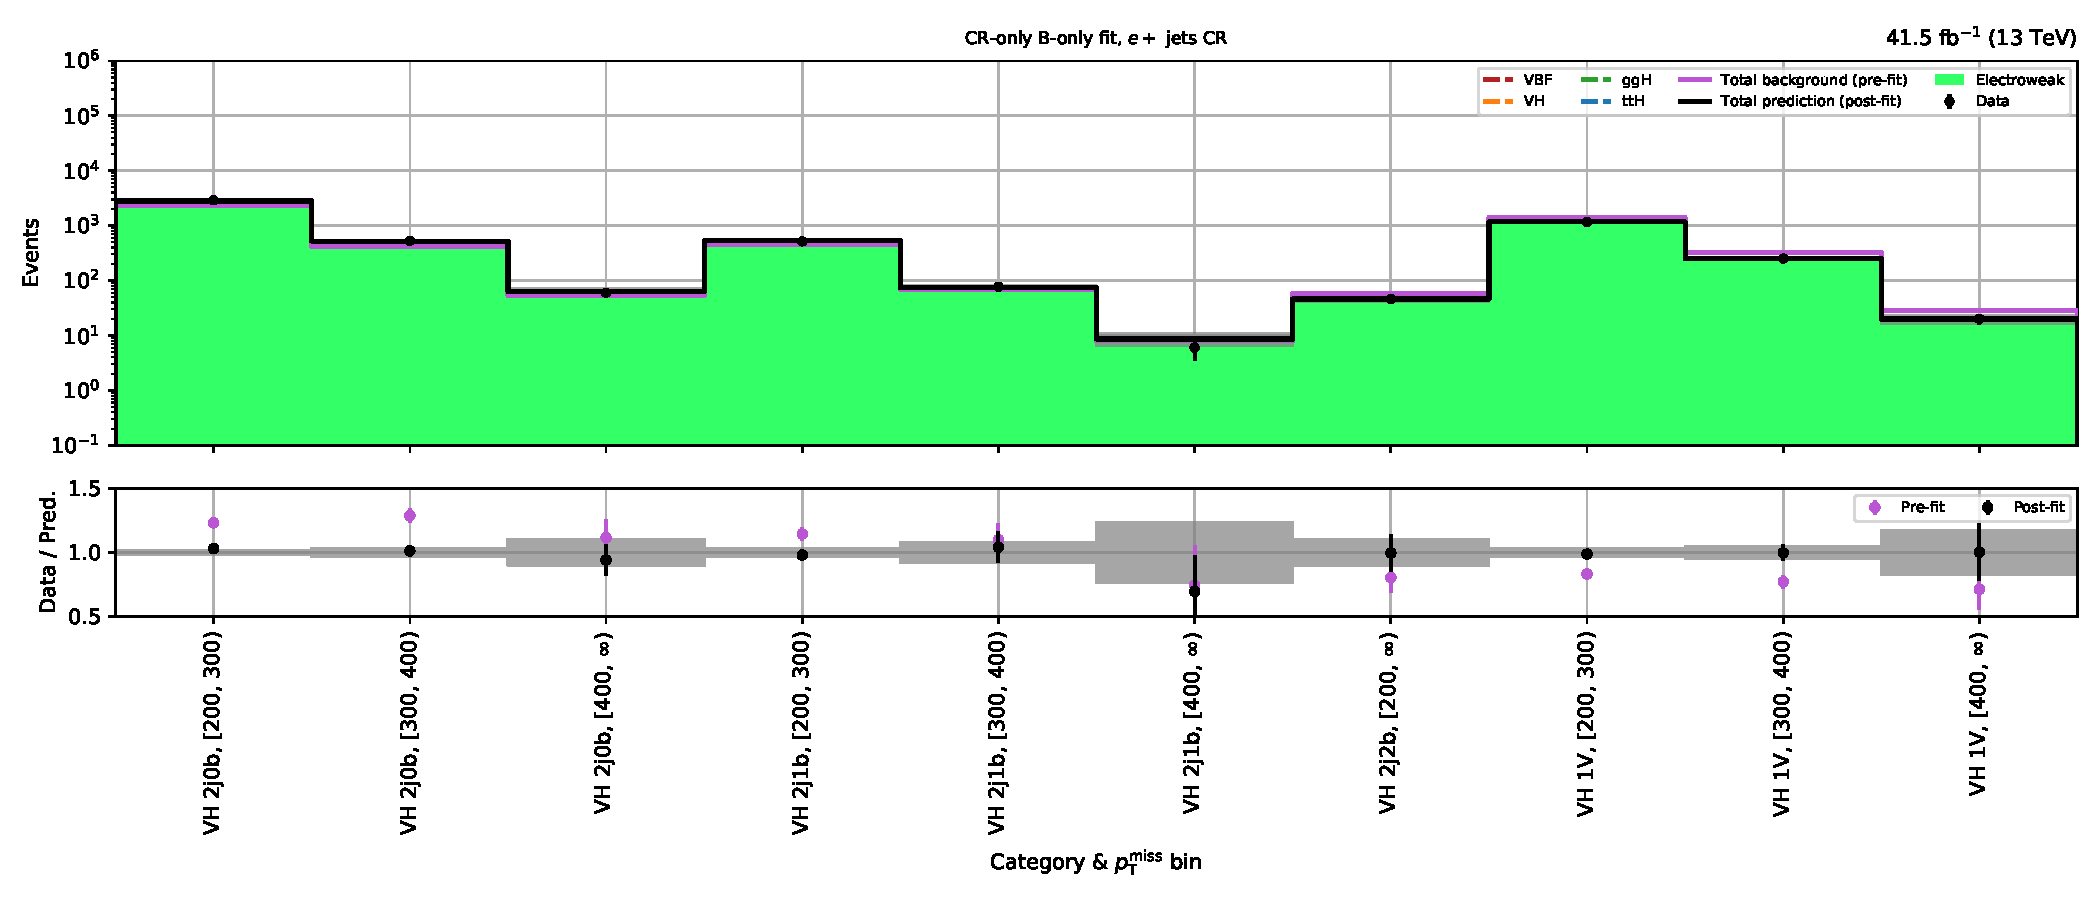
\includegraphics[width=\textwidth]{chapters/higgstoinv/figures/mountain_ranges/2017/VH/Wenu_tree_fit_b-abs_values_VH_cats.pdf}
        \caption{\VH --- \singleEleCr \gls{CR} (2017)}
    \end{subfigure}
    \caption[Post-fit yields for each category and \ptmiss bin in the single lepton control regions of the \VH categories for the 2017 dataset]{Post-fit yields for each category and \ptmiss bin in the single lepton \glspl{CR} of the \VH categories for the 2017 dataset. The total background pre-fit and post-fit is compared to data in the lower panel of each subfigure.}
    \label{fig:htoinv_mountain_range_2017_single_lep_VH}
\end{figure}

\clearpage

The fit performs adequately in bringing the simulation in closer agreement to the data, despite large initial disagreement in some bins. All of the bins are sufficiently populated, such that the uncertainty on the prediction is small in most cases. The predicted \acrshort{sm} background counts in the signal region from Tab.~\ref{tab:yields_SR_CR_only_2017} further corroborates the results as the yields are close to, if not above than the data in several bins.


%=========================================================


\subsection{\texorpdfstring{\ztonunupjets}{Z to nunu + jets} background estimation}
\label{subsubsec:htoinv_znunu_bkg}

The irreducible background from invisibly decaying \PZ bosons is estimated in the same manner as the lost lepton background. A rate parameter $a_{\ztonunu}$ ties together the dilepton \glspl{CR}, the photon \gls{CR}, and the signal region. The yields from simulation are scaled by the best fit value of the parameter, obtained during the simultaneous fit to the analysis regions. As with the lost lepton background, event categorisation is the same in these regions, allowing the predictions to be derived independently for each category and \ptmiss bin.

For the \ttH categories, the \singlePhotonCr \gls{CR} is not used for the \ztonunu prediction. The region is leveraged by the \VH categories, however. In addition to the electroweak background dominated by \gammapjets simulation, the \acrshort{qcd} multijet presence---consisting of \glspl{jet} misidentified as photons---in the photon \gls{CR} is estimated by way of a data-driven purity measurement. This is detailed extensively in Chpt.~\ref{subsubsec:htoinv_photon_purity}. The results of a \gls{CR}-only fit to data for the 2017 dataset are shown as an example in Chpt.~\ref{subsubsec:htoinv_zinv_CR_only_fit}.


%=========================================================


\subsubsection{Photon purity measurement for the \texorpdfstring{\singlePhotonCr}{photon} control region}
\label{subsubsec:htoinv_photon_purity}

Photons are reconstructed from clusters in the \acrshort{ecal}. They can usually be discriminated from other sources leaving \acrshort{ecal} deposits due to the properties of the deposits themselves, as well as the lack of other signatures that typically belong to other particles. However, this method is imperfect, and occasionally other particles will be incorrectly identified as photons (which are known as ``fakes''). The leading sources of fake photons is from \acrshort{qcd} multijet events where a \gls{jet} is misidentified as such. Due to the high cross section of the process, even a small rate of fake photons becomes important to consider.

In order to separate real photons from fakes in the \singlePhotonCr \gls{CR}, a purity measurement is performed. The purity is defined as the fraction of reconstructed photons that are from an isolated photon emerging from the hard scatter of the event, rather than a fake. The variable $\sieie$ is able to distinguish between real and fake photons with sufficient power. A peak with a hard cut off at $\sieie \approx \text{0.01}$ is observed for real photons, while fakes possess a less pronounced peak and much slower decline above that threshold. As such, a template fit is performed to the distribution in data to extract the purity.

As inputs to the fit, photons in data are selected by applying the medium identification requirements from Tab.~\ref{tab:htoinv_photon_ID_barrel} with the exception of $\sieie$ to observe the full range. Photons from \singlePhotonCr simulation are selected with the same criteria and are used to define the real photon template. A fake photon template is obtained from data by requiring at least one of the isolation criteria from the medium ID in Tab.~\ref{tab:htoinv_photon_ID_barrel} to be unfulfilled. This ensures the photons from this set do not overlap with the real photons from data.

The templates are derived in separate bins of photon \pt, and the purity measurement is performed separately for each data taking year. The following event selection is applied:

\medskip
\begin{easylist}[itemize]
    \cutflowlistprops
    & Photon trigger requirement for the respective dataset from Tab.~\ref{tab:htoinv_photon_pd_triggers}
    & \ptmiss filters from Chpt.~\ref{subsec:htoinv_other_filters}
    & $\ptmiss < \text{60}\GeV$
    & At least one jet with $\pt > \text{80}\GeV$ and $\abseta < \text{2.4}$, separated from photons with $\Delta R > \text{0.4}$
    & If a second jet is present, it is required to have $\abseta < \text{2.4}$ and also be separated from photons with $\Delta R > \text{0.4}$
    & $\HT > \text{200} \GeV$
\end{easylist}

\medskip

\noindent{}A combination of cuts are used to select photons appropriately and ensure the phase space resembles that of the \singlePhotonCr \gls{CR}. The shapes of the real and fake templates are fit to the data using a likelihood function in the range $\text{0.004} \leq \sieie \leq \text{0.02}$. Two examples, for the lowest and highest \pt bins from the 2017 dataset, are shown in Fig.~\ref{fig:htoinv_photon_purity_fits}.

\begin{figure}[H]
    \centering
    \begin{subfigure}[b]{0.42\textwidth}
        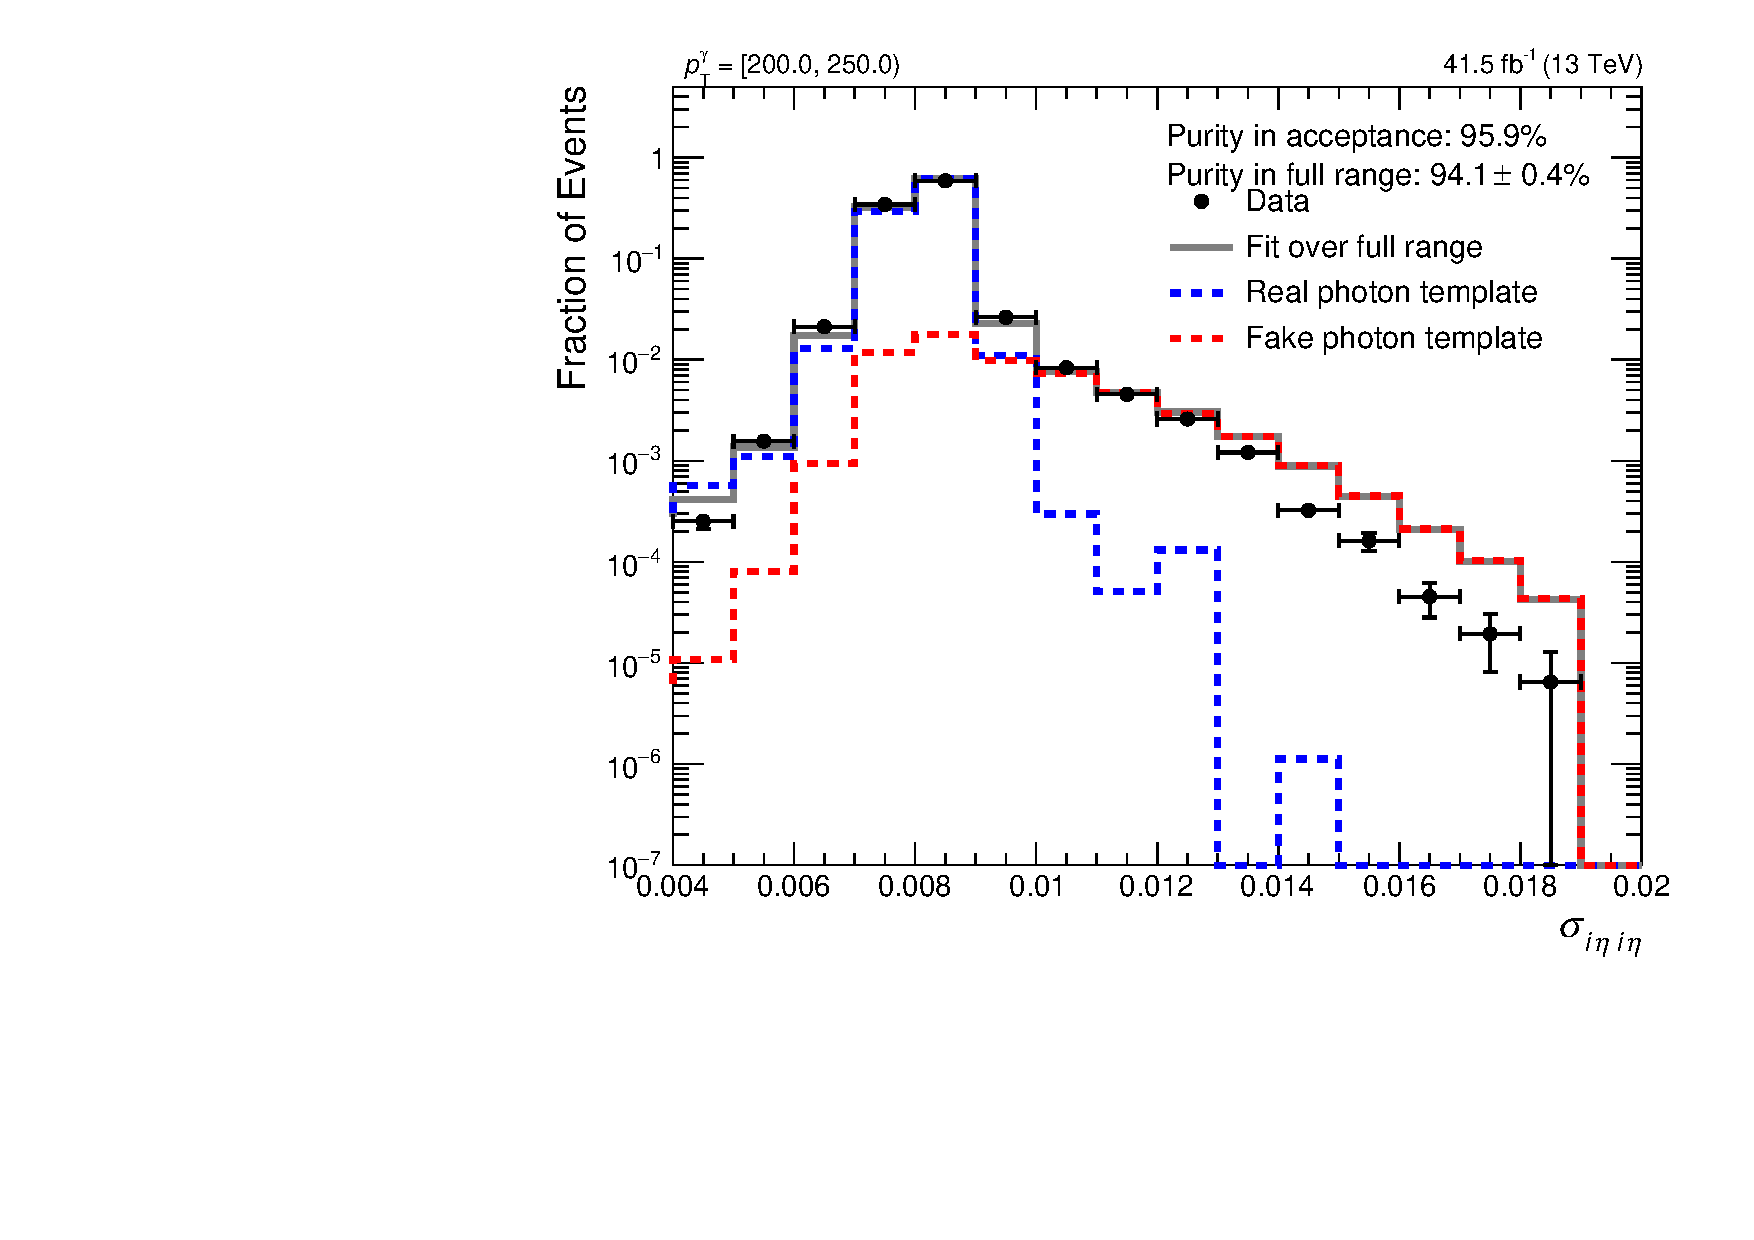
\includegraphics[width=\textwidth]{figures/photon_purity/2017/fit_200.0_to_250.0.pdf}
        \caption{$\text{200} < \pt^{\Pphoton} < \text{250\GeV}$}
    \end{subfigure}
    \hspace{0.1\textwidth}
    \begin{subfigure}[b]{0.42\textwidth}
        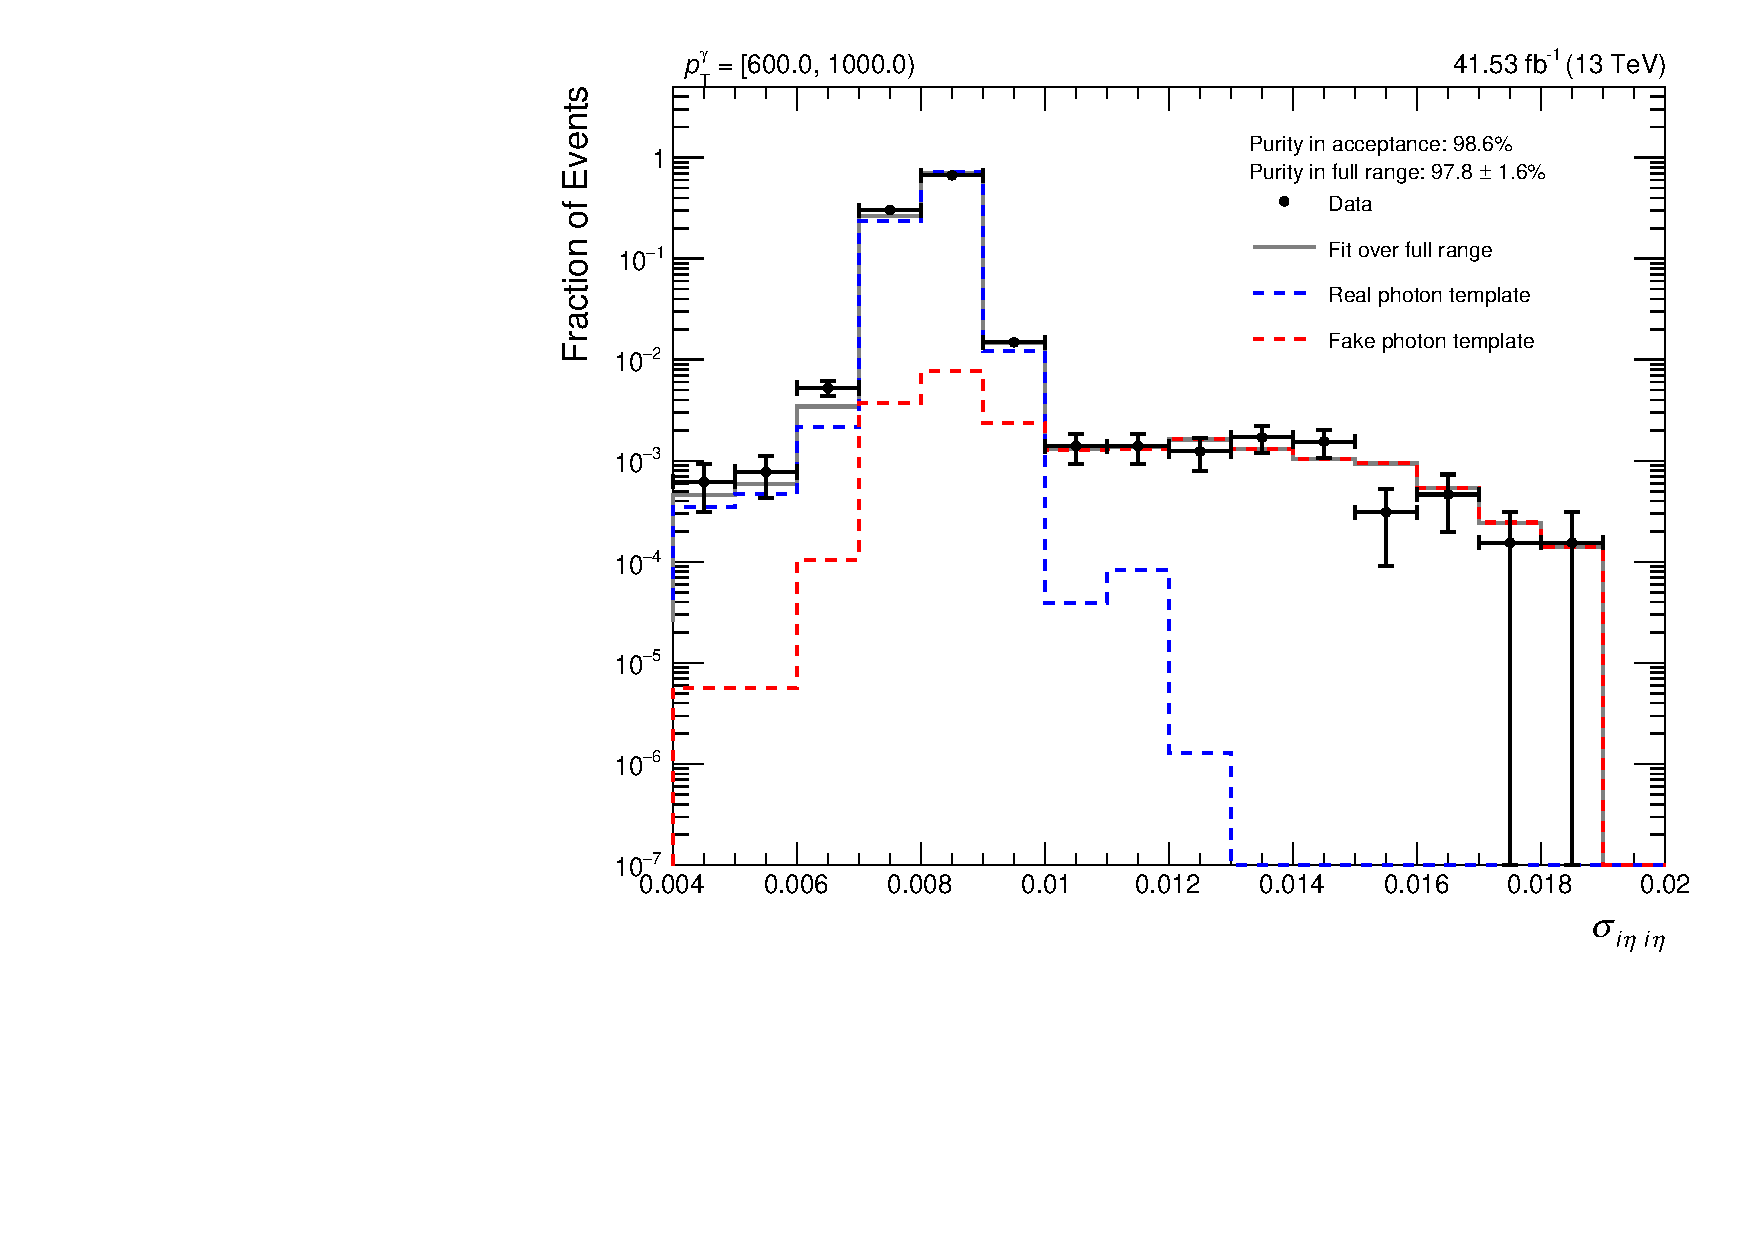
\includegraphics[width=\textwidth]{figures/photon_purity/2017/fit_600.0_to_1000.0.pdf}
        \caption{$\text{600} < \pt^{\Pphoton} < \text{1000\GeV}$}
    \end{subfigure}
    \caption[Fits of real and fake photon templates to data in the \sieie spectrum]{Fits of real and fake photon templates to data in the \sieie spectrum. Two bins of $\pt^{\Pphoton}$ are illustrated, demonstrating the different shapes of the templates and data, with the purity over the full range and within acceptance ($\sieie \leq \text{0.01}$) noted.}
    \label{fig:htoinv_photon_purity_fits}
\end{figure}

It can be seen that the data resembles the real template at low values of \sieie with the fake template dominating at larger values. Each fit captures the features of both templates appropriately. By calculating the purity within acceptance (i.e., $\sieie \leq \text{0.01}$ as given by the medium ID requirement), the \emph{impurity} can be derived as a function of photon \pt. An exponential function is fitted to interpolate within the range that also serves to extrapolate above it. Fig.~\ref{fig:htoinv_photon_impurity} illustrates the impurity versus photon \pt for each data taking year. A 25\,\% uncertainty around the fit is assumed to account for effects related to the binning of the \sieie distribution.

\begin{figure}[htbp]
    \centering
    \begin{subfigure}[b]{0.32\textwidth}
        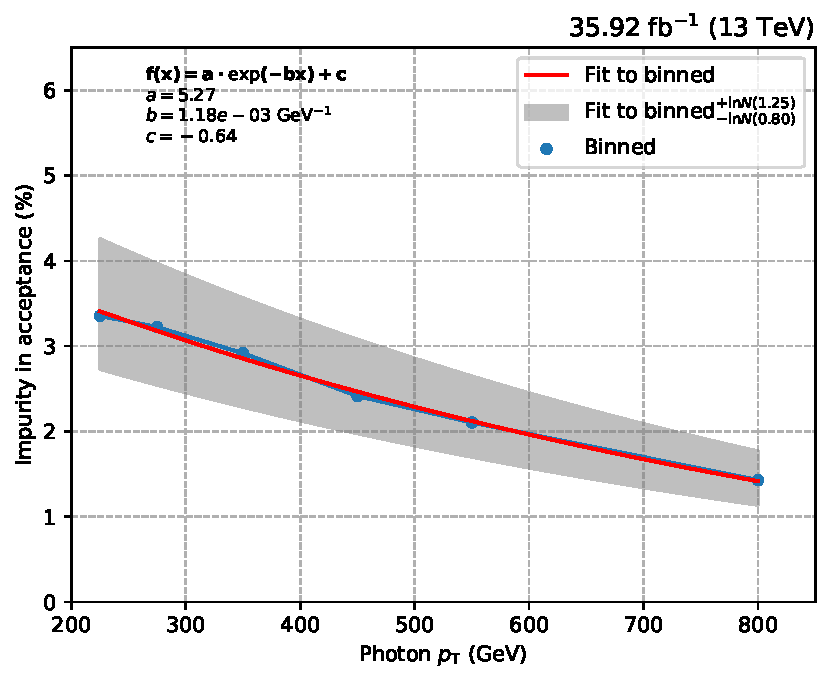
\includegraphics[width=\textwidth]{figures/photon_purity/2016/impurity_plot_2016.pdf}
        \caption{2016}
    \end{subfigure}
    \hfill
    \begin{subfigure}[b]{0.32\textwidth}
        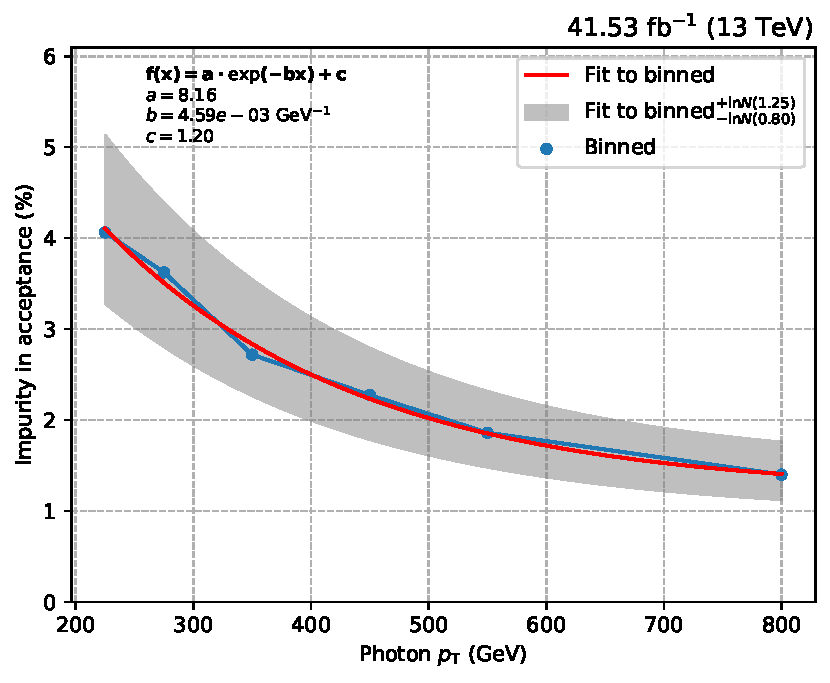
\includegraphics[width=\textwidth]{figures/photon_purity/2017/impurity_plot_2017.pdf}
        \caption{2017}
    \end{subfigure}
    \hfill
    \begin{subfigure}[b]{0.32\textwidth}
        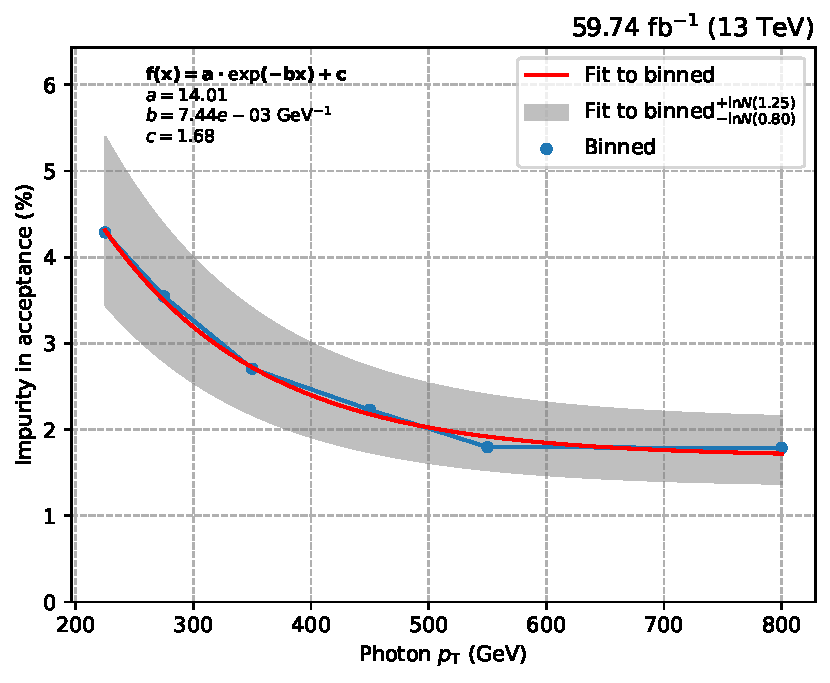
\includegraphics[width=\textwidth]{figures/photon_purity/2018/impurity_plot_2018.pdf}
        \caption{2018}
    \end{subfigure}
    \caption[The fraction of impure photons in data as a function of \pt for each data taking year in Run-2]{The fraction of impure photons in data as a function of \pt for each data taking year in Run-2. An exponential is fit to the binned data with a 25\,\% uncertainty assigned to account for binning effects.}
    \label{fig:htoinv_photon_impurity}
\end{figure}

The impurity expectedly decreases as a function of the photon \pt. Harder particles are usually reconstructed better in the detector with more isolated deposits in the calorimeters while maintaining excellent momentum resolution. Several factors affecting the data quality in 2017 and 2018 could have led to the larger fake rates in the distributions, such as pre-firing and the HEM issue. Few issues were present in 2016. \acrlong{mc} in each year may have also impacted the measurement as the modelling parameters often differ between years.

In the analysis, the purity measurement is used to estimate the \acrshort{qcd} multijet background in the \singlePhotonCr \gls{CR}, replacing the contribution from \acrshort{mc}. For each event in data that enters the region, a \acrshort{qcd} multijet pseudo-event is created with the same properties---notably \ptmiss and photon \pt. The value of the impurity calculated from the photon's \pt weights the event. The new \acrshort{qcd} background is therefore generated with the same shape as the data and weighted to represent the rate of non-prompt photons. A 25\,\% uncertainty is attributed to the normalisation of the yield.

% See https://root.cern/doc/master/classTFractionFitter.html for implementation


%=========================================================


\subsubsection{Results from a control region-only fit}
\label{subsubsec:htoinv_zinv_CR_only_fit}

Distributions of the dilepton and photon \glspl{CR} from the \gls{CR}-only fit are shown in Figs.~\ref{fig:htoinv_mountain_range_2017_dilep_CRs_ttH} and \ref{fig:htoinv_mountain_range_2017_dilep_CRs_VH} in the \ttH and \VH categories, respectively, for the 2017 dataset. Corresponding event counts, along with the rate parameters, can be found in Tab.~\ref{tab:htoinv_rate_params_2017_zinv}. The predicted invisible \PZ background in the signal region, for comparisons to the observed data, is tabulated in Tab.~\ref{tab:yields_SR_CR_only_2017}. Equivalent figures for the other data taking periods are accessible in Apps.~\ref{sec:pre_post_fit_plots_ttH_CRs} and \ref{sec:pre_post_fit_plots_VH_CRs} for the \ttH and \VH categories, respectively.

\begin{figure}[htbp]
    \centering
    \begin{subfigure}[b]{\textwidth}
        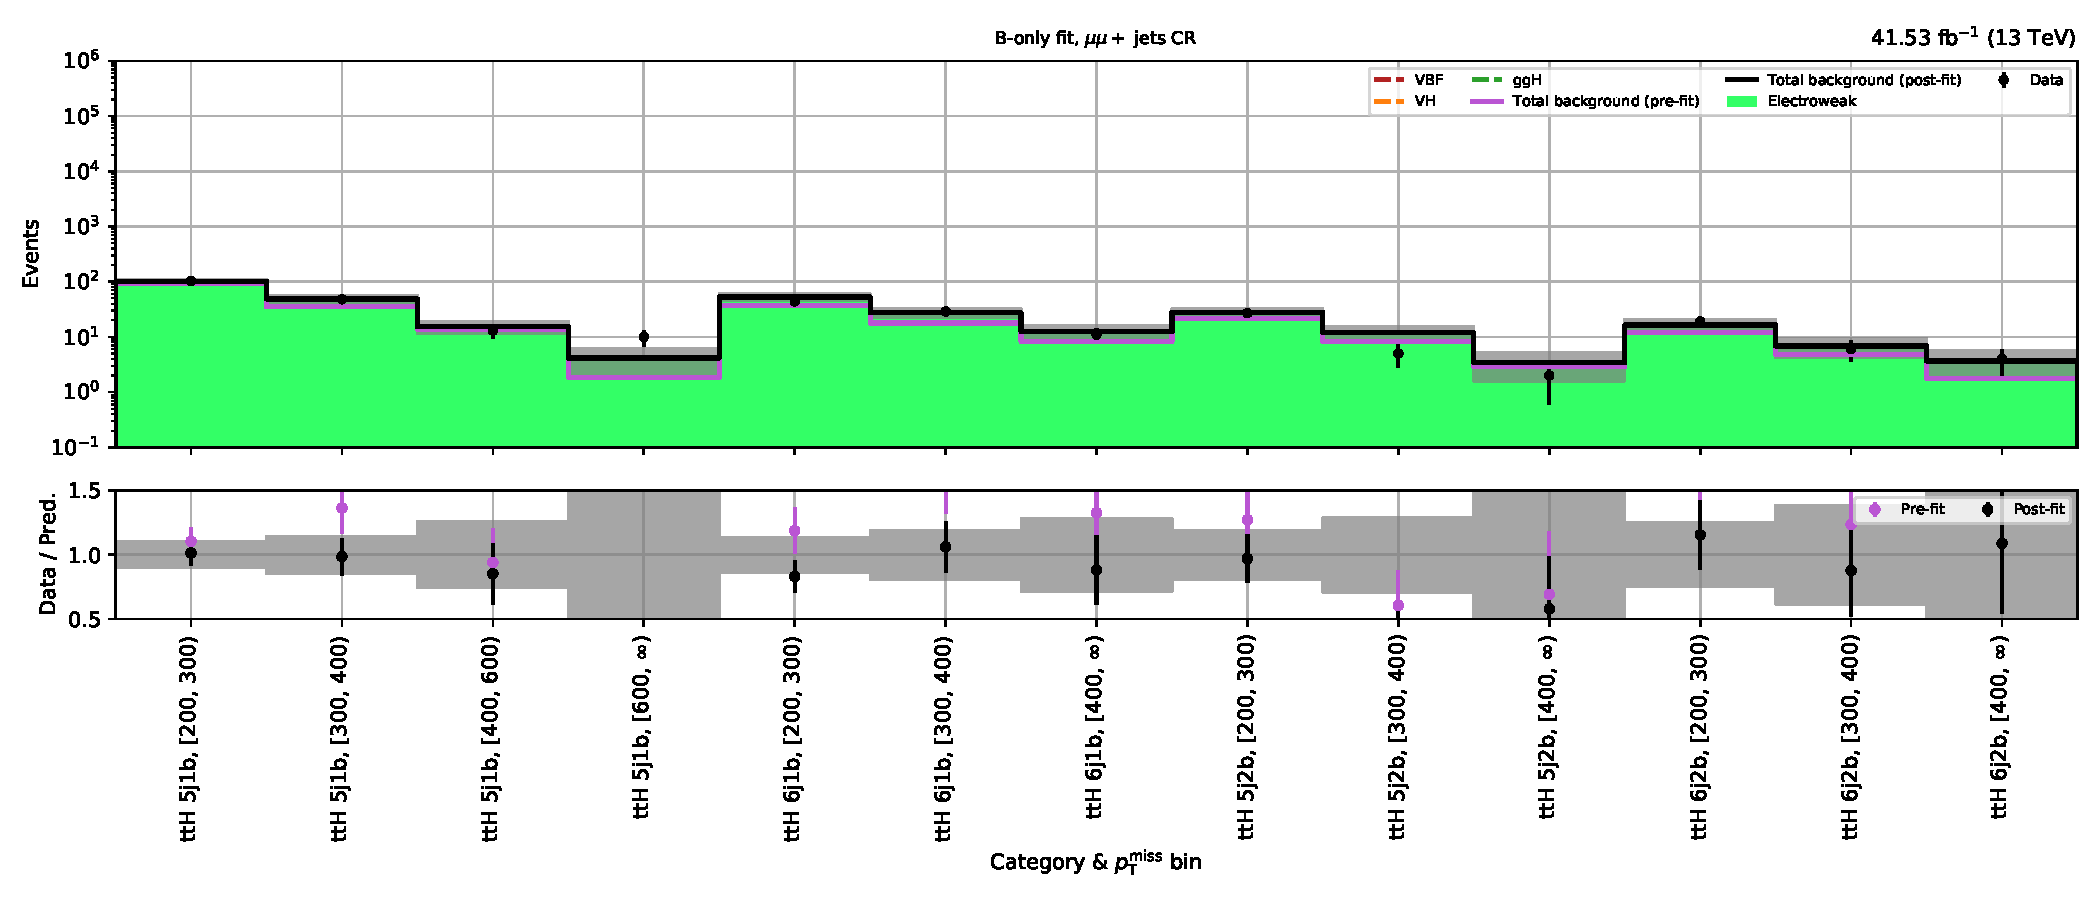
\includegraphics[width=\textwidth]{chapters/higgstoinv/figures/mountain_ranges/2017/ttH/Zmumu_tree_fit_b-abs_values_ttH_cats.pdf}
        \caption{\ttH --- \doubleMuCr \gls{CR} (2017)}
    \end{subfigure}
    \hfill
    \begin{subfigure}[b]{\textwidth}
        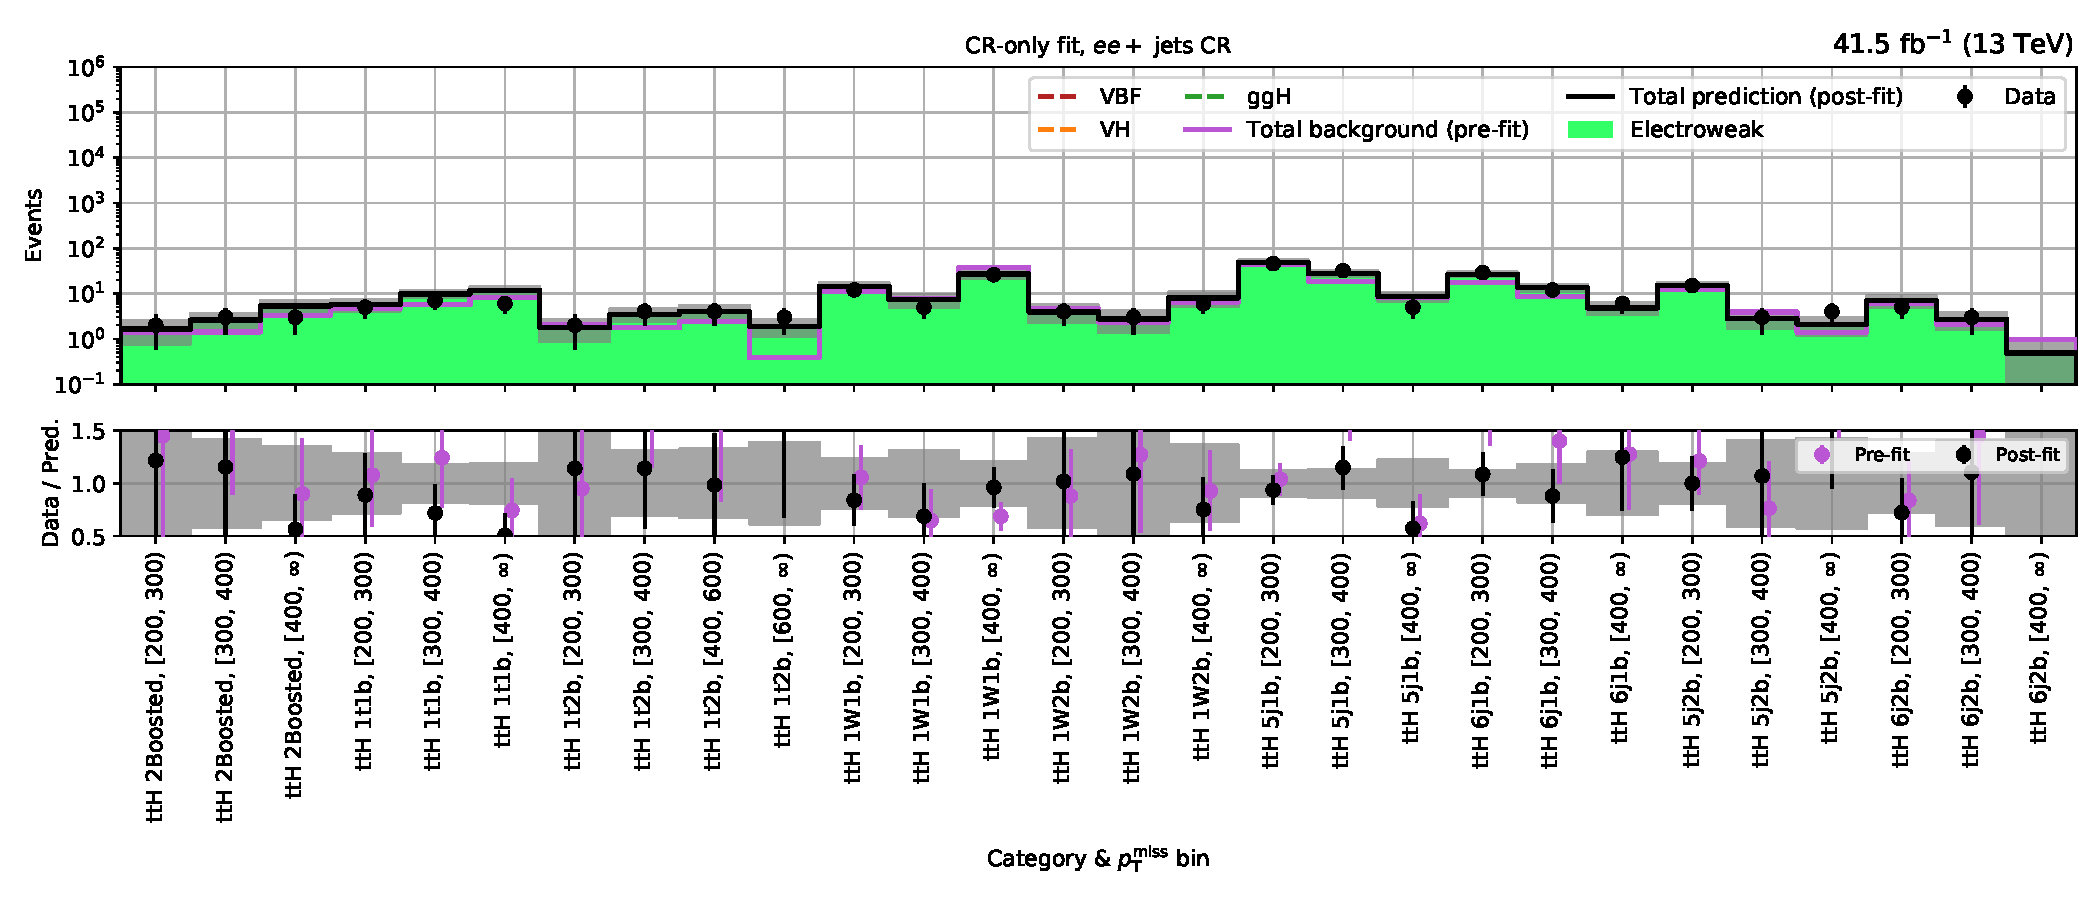
\includegraphics[width=\textwidth]{chapters/higgstoinv/figures/mountain_ranges/2017/ttH/Zee_tree_fit_b-abs_values_ttH_cats.pdf}
        \caption{\ttH --- \doubleEleCr \gls{CR} (2017)}
    \end{subfigure}
    \caption[Post-fit yields for each category and \ptmiss bin in the dilepton control regions of the \ttH categories for the 2017 dataset]{Post-fit yields for each category and \ptmiss bin in the dilepton \glspl{CR} of the \ttH categories for the 2017 dataset. The total background pre-fit and post-fit is compared to data in the lower panel of each subfigure.}
    \label{fig:htoinv_mountain_range_2017_dilep_CRs_ttH}
\end{figure}

\begin{figure}[htbp]
    \centering
    \begin{subfigure}[b]{0.9\textwidth}
        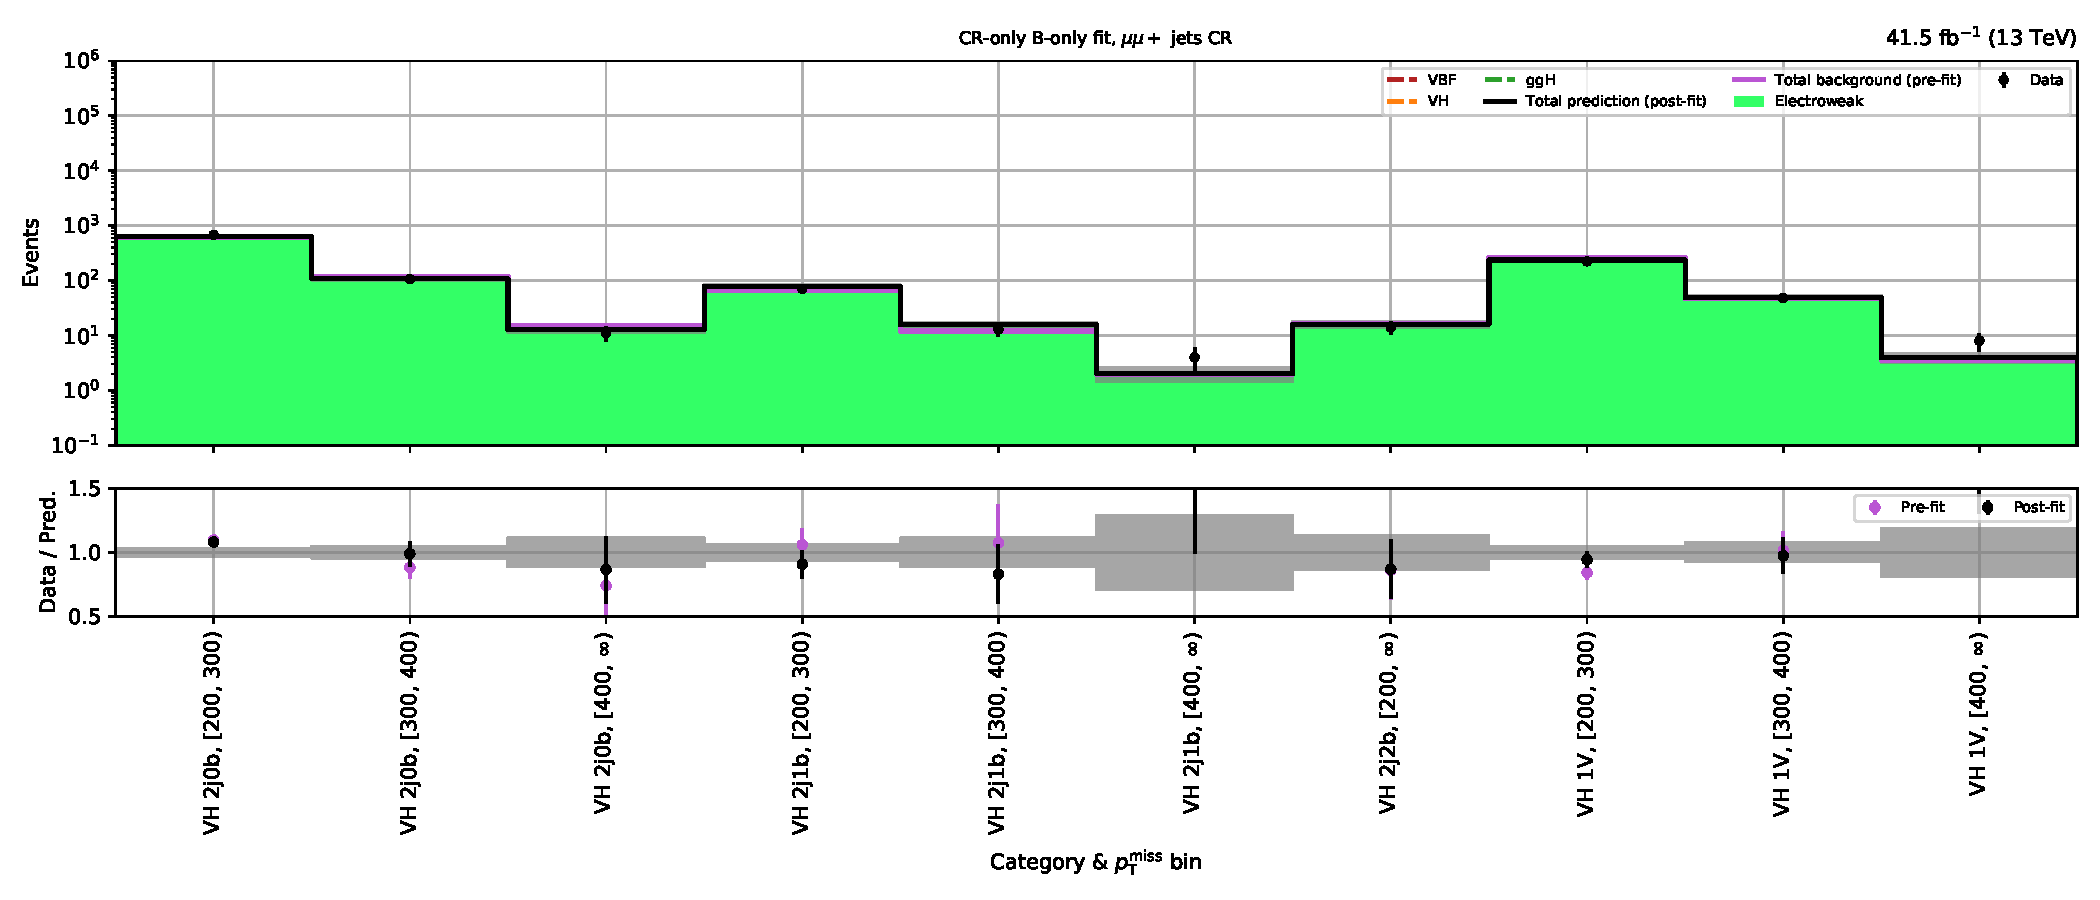
\includegraphics[width=\textwidth]{chapters/higgstoinv/figures/mountain_ranges/2017/VH/Zmumu_tree_fit_b-abs_values_VH_cats.pdf}
        \caption{\VH --- \doubleMuCr \gls{CR} (2017)}
    \end{subfigure}

    \begin{subfigure}[b]{0.9\textwidth}
        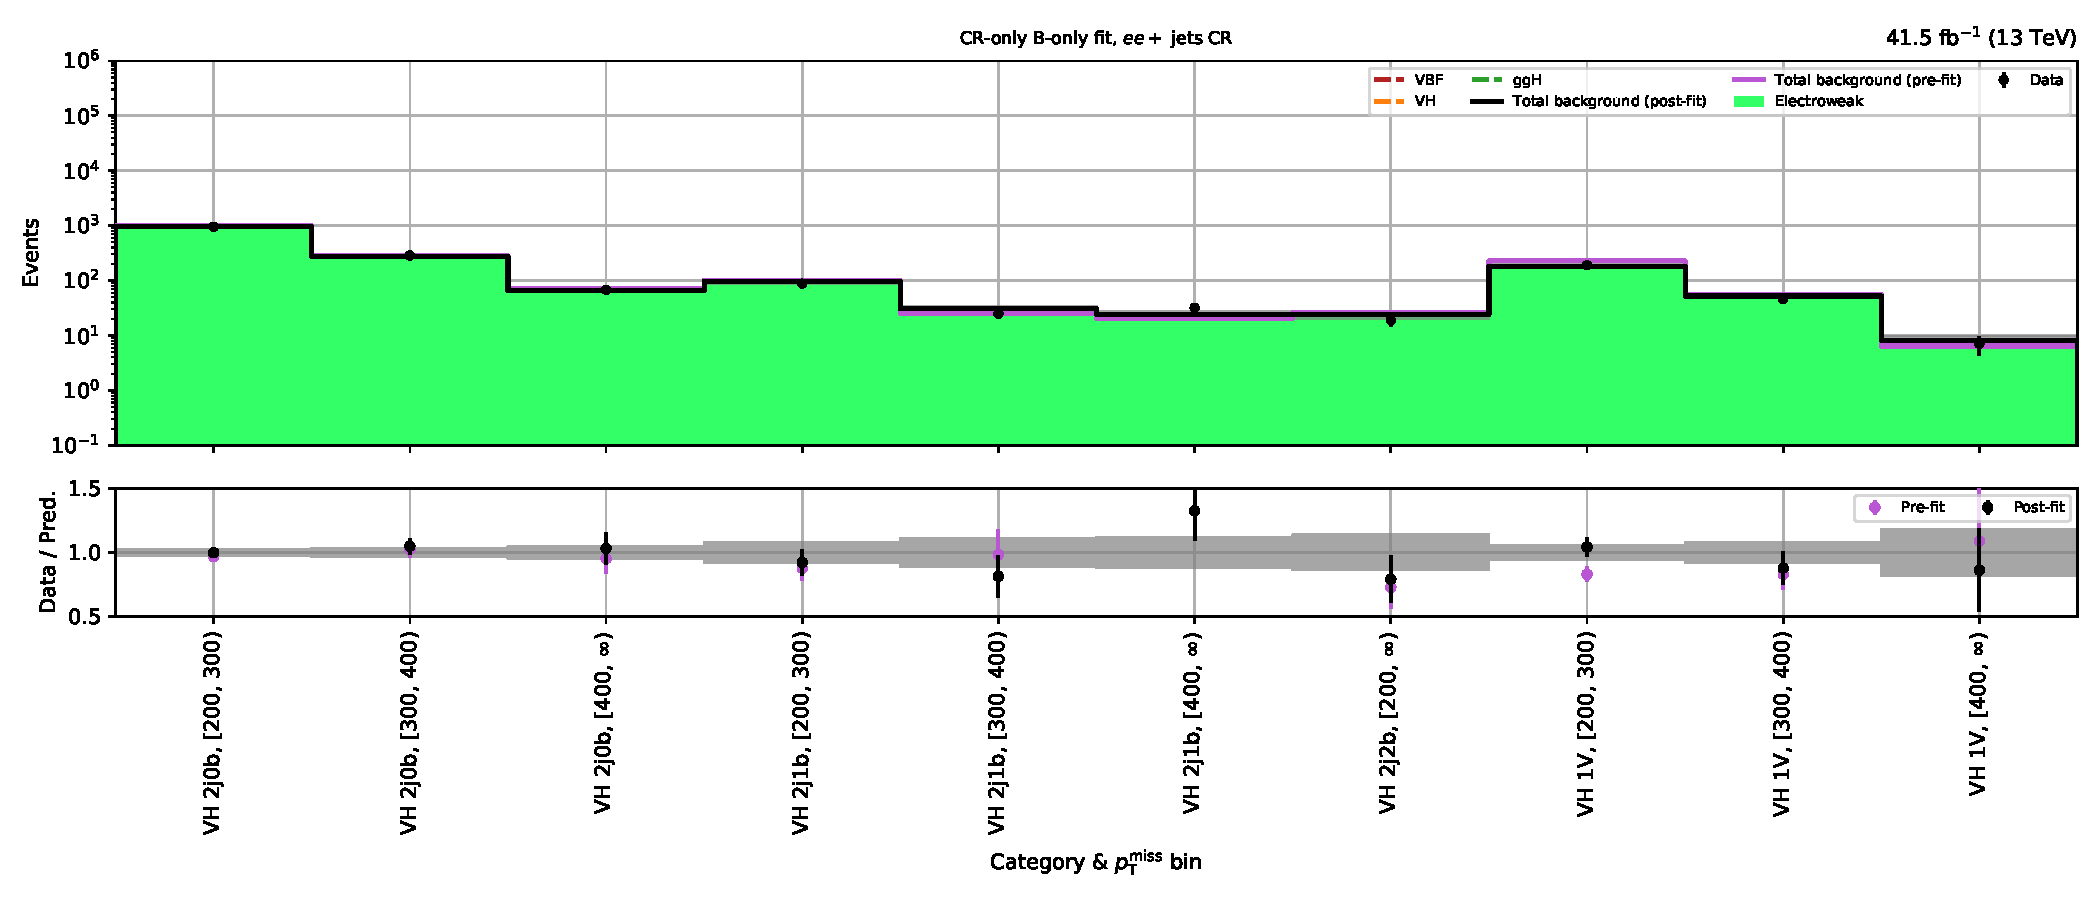
\includegraphics[width=\textwidth]{chapters/higgstoinv/figures/mountain_ranges/2017/VH/Zee_tree_fit_b-abs_values_VH_cats.pdf}
        \caption{\VH --- \doubleEleCr \gls{CR} (2017)}
    \end{subfigure}

    \begin{subfigure}[b]{0.9\textwidth}
        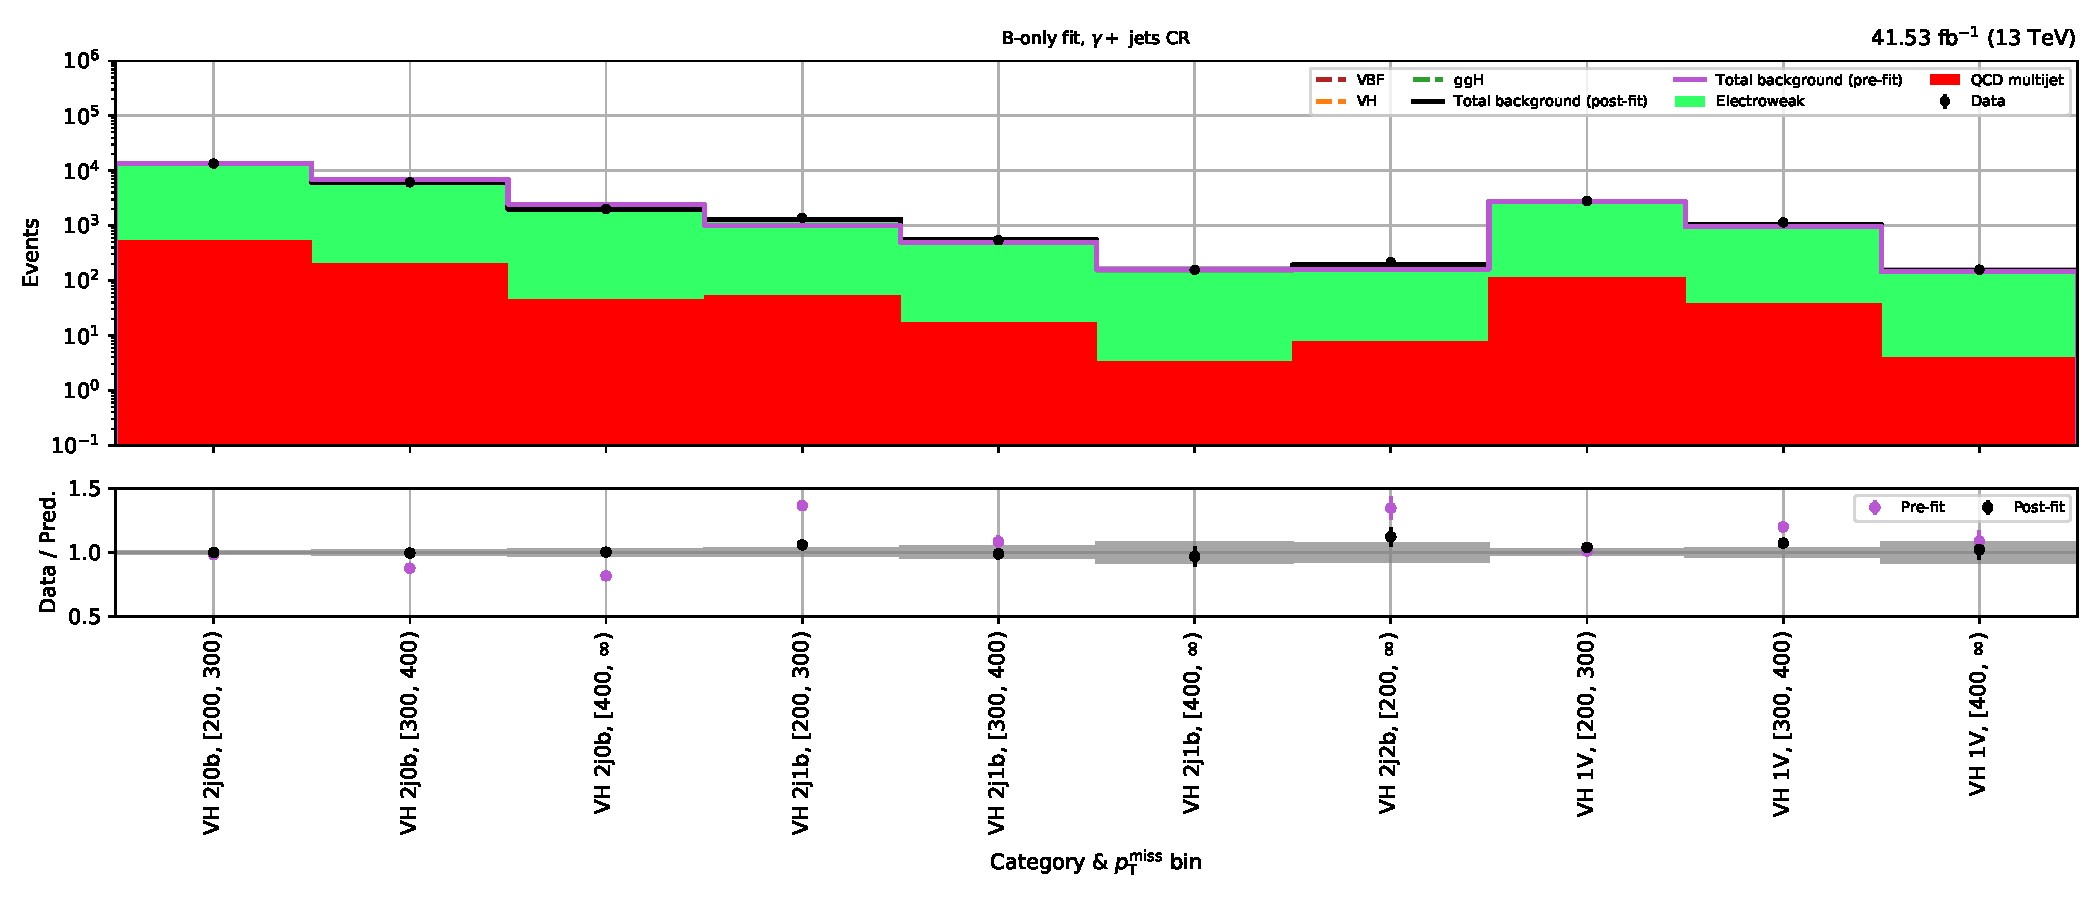
\includegraphics[width=\textwidth]{chapters/higgstoinv/figures/mountain_ranges/2017/VH/Photon_tree_fit_b-abs_values_VH_cats.pdf}
        \caption{\VH --- \singlePhotonCr \gls{CR} (2017)}
    \end{subfigure}
    \caption[Post-fit yields for each category and \ptmiss bin in the dilepton and photon control regions of the \VH categories for the 2017 dataset]{Post-fit yields for each category and \ptmiss bin in the dilepton and photon \glspl{CR} of the \VH categories for the 2017 dataset. The total background pre-fit and post-fit is compared to data in the lower panel of each subfigure.}
    \label{fig:htoinv_mountain_range_2017_dilep_CRs_VH}
\end{figure}

Despite the low yields in the \ttH categories, the fit is able to correct the simulated background closer the observed data in most of the bins. A comparable result is achieved in the \VH categories. The highly populated \singlePhotonCr \gls{CR} adds a powerful additional constraint to the prediction; an extremely useful inclusion given \ztonunu is comfortably the dominant background for the \VH channel. With \acrshort{qcd} contributing under 5\,\% to the total yield in the photon region, convergence of the fit is naturally driven by the electroweak processes.


%=========================================================


\subsection{QCD multijet background estimation}
\label{subsec:htoinv_qcd_multijet_bkg}

The effects of \gls{jet} mismeasurements are difficult to quantify. With a final state of several \glspl{jet} in the \acrshort{qcd} multijet process, little, or even no \ptvecmiss is expected. Therefore, a single mismeasured \gls{jet} will introduce artificial \ptvecmiss in the direction of that jet. A low $\mindphiAB{\mathrm{j}}{\ptvecmiss}$ is therefore expected. Though it is not just this background that suffers as \glspl{jet} from ``cleaner'' processes may also be affected. But those with real \ptmiss in an event (e.g., $\ztonunupjets$) are unlikely to be significantly influenced by one stray object. The enormous cross section of \acrshort{qcd} multijet amplifies the problem, making the process as a whole more sensitive to, e.g., fluctuations in the calorimeter response that would affect the energy measurement.

Contributions to the signal region from \acrshort{qcd} multijet events should be adequately suppressed by the analysis-level selection requirements. However, it is still a process that must be accurately accounted for considering its rate of production at \acrshort{cms}. A metric by which to estimate the number of events a dataset should require is by calculating the equivalent luminosity:
\begin{equation}
    \lumi_{\mathrm{eq.}} = \frac{N_{\mathrm{events}}}{\sigma}
    \label{eq:equivalent_lumi}
\end{equation}
A general rule is that the equivalent luminosity of a given dataset should be comparable to, or even exceed, that of the data collected by the experiment. Since the \acrshort{qcd} multijet process has a very large cross section, simulating the required number of events to match the luminosity of the data recorded during Run-2 is not feasible.

To estimate the presence of \acrshort{qcd} in the signal region, a data driven approach is taken utilising the sidebands defined in Chpt.~\ref{subsubsec:htoinv_sidebands}. Then, the application of the sidebands to derive the predicted event counts in the signal region is outlined in Chpt.~\ref{subsubsec:htoinv_qcd_pred_SR}. This is derived separately for each channel and data taking year.


%=========================================================


\subsubsection{Sidebands to the signal region}
\label{subsubsec:htoinv_sidebands}

Several kinematic cuts in the analysis are designed to reject \acrshort{qcd} in the signal region. So by inverting and tightening one or more of them, it is possible to construct multijet-enriched regions known as \emph{\glspl{SB}}. The sideband is defined for the \ttH channel by inversions on the angular variables \omegaTilde and \dphiFj:

\medskip
\begin{easylist}[itemize]
    \easylistprops
    & \ttH sideband: $\omegaTilde < \text{0.2}$, $\dphiFj \leq \text{0.5}$
\end{easylist}

\medskip

\noindent{}The signal region is defined by $\omegaTilde > \text{0.3}$ and $\dphiFj > \text{0.5}$ as in Tab.~\ref{tab:htoinv_categories}. Otherwise, the same selection applied to the signal region is also done so for the sidebands. Yields from all of the \ttH categories are combined to form the sidebands as statistical limitations would otherwise ensue.

Events with a \VH topology, being characterised by a dijet pair or single fat jet recoiling from the \ptvecmiss, naturally have a large \mindphiJetMet. Obtaining a multijet enriched sideband by inverting this variable was therefore not possible. The sidebands inverted in \omegaTilde also contained little \acrshort{qcd} to extrapolate from. Therefore, a single sideband was created from the 2j0b category that inverts \mindphi, \omegaTilde (tightly, as with \ttH), and the dijet mass requirement from Tab.~\ref{tab:htoinv_categories}:

\medskip
\begin{easylist}[itemize]
    \easylistprops
    & \VH sideband: $\omegaTilde < \text{0.2}$, $\dphiFj \leq \text{0.5}$, $\mjj \notin [\text{65}, \text{105})$
\end{easylist}

\medskip

\noindent{}The latter inversion populates the sideband sufficiently with multijet events. This sideband is utilised by all \VH categories, as while the 1V category does not enforce the same dijet mass window, the soft drop mass requirement for the boosted \PVec-tagged \gls{jet} is a suitable proxy. Inclusion of \glspl{bjet} in the 2j1b and 2j2b categories reduces the multijet content of potential sidebands significantly. This is the reason these categories also utilise the sideband constructed from 2j0b.

Fig.~\ref{fig:htoinv_sb_yields_combRun2} illustrates the \ptmiss distributions in the \ttH and \VH \glspl{SB} after the analysis-level selections with the full Run-2 dataset. Background estimation is performed separately for each year due to the differing running conditions, detector configuration, and the different effects or features seen in the data.

\begin{figure}[htbp]
    \centering
    \begin{subfigure}[b]{0.45\textwidth}
        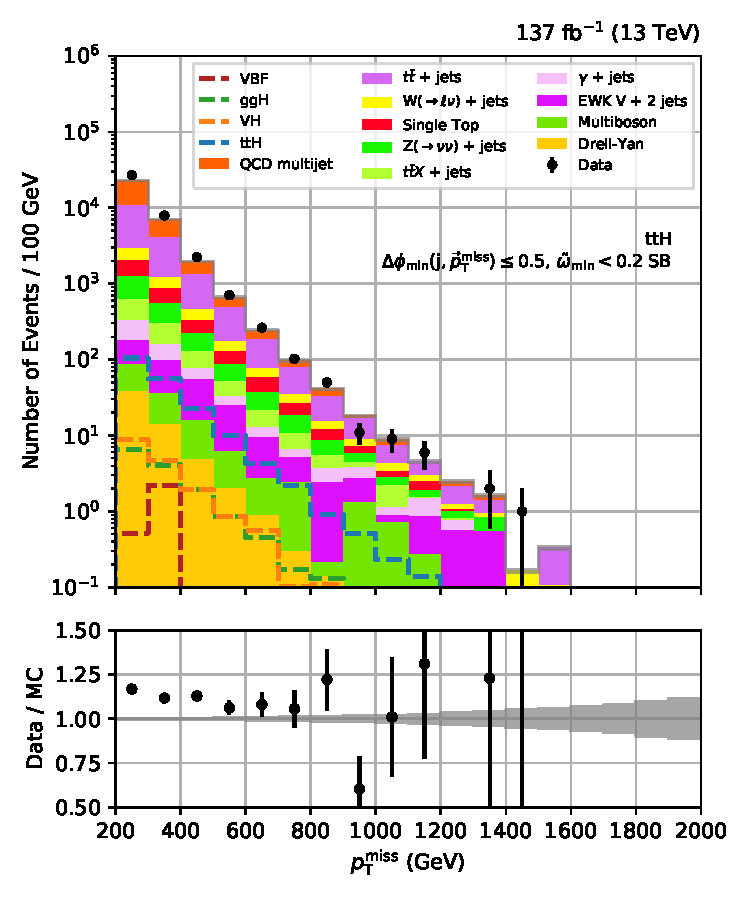
\includegraphics[width=\textwidth]{figures/region_plots/full_Run2/sideband_0/ttH.pdf}
        \caption{\ttH}
    \end{subfigure}
    \hspace{0.05\textwidth}
    \begin{subfigure}[b]{0.45\textwidth}
        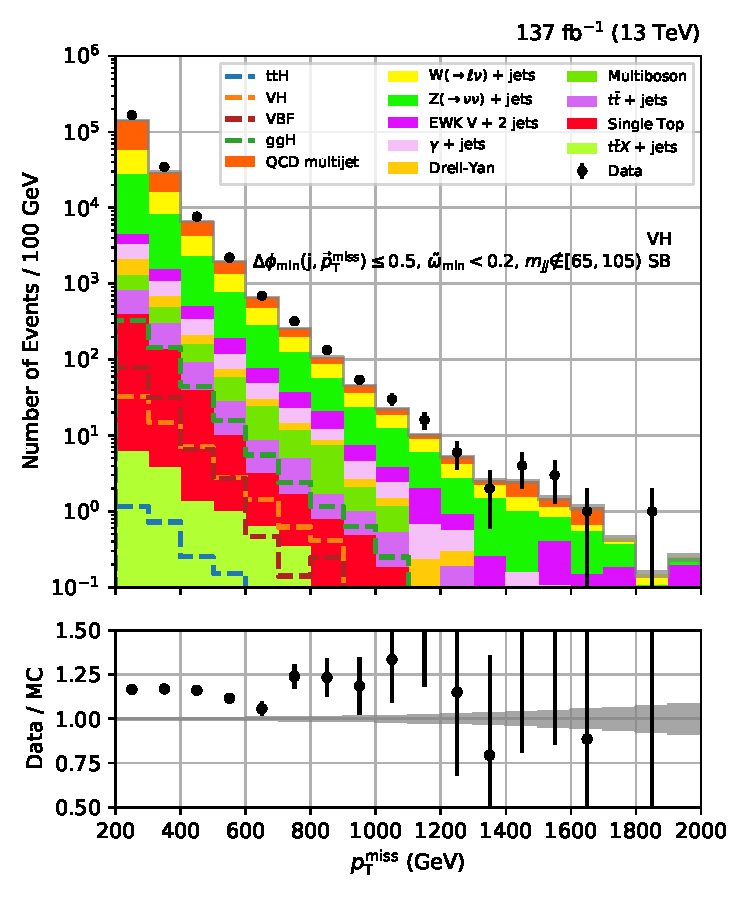
\includegraphics[width=\textwidth]{figures/region_plots/full_Run2/VH_sideband/VH.pdf}
        \caption{\VH}
    \end{subfigure}
    \caption[Data--simulation comparisons of the \ptmiss distribution in the \ttH and \VH sidebands, aggregated over the full Run-2 dataset]{Data--simulation comparisons of the \ptmiss distribution in the \ttH and \VH sidebands, aggregated over the full Run-2 dataset.}
    \label{fig:htoinv_sb_yields_combRun2}
\end{figure}


%=========================================================


\subsubsection{Prediction in the signal region}
\label{subsubsec:htoinv_qcd_pred_SR}

A \gls{CR}-only fit is performed without multijet simulation to extract the rate parameters ($a$ from Eq.~\ref{eq:likelihood_CRs}) that scale the electroweak backgrounds in the signal region. Applying these also to the corresponding backgrounds in the sidebands changes the event distribution and hence the data--\acrshort{mc} agreement. The excess in data in a sideband is assumed to arise solely from multijet events, and as such the difference between data and the non-multijet background is attributed to \acrshort{qcd} (denoted as $N_{\mathrm{SB}}^{\mathrm{QCD}}$).

\acrshort{qcd} in the signal region $N_{\mathrm{pred.}}^{\mathrm{QCD}}$ (corresponding to $c_{\mathrm{QCD}}$ in Eq.~\ref{eq:likelihood_SR}) is predicted in each category and \ptmiss bin as follows:
\begin{equation}
    N_{\mathrm{pred.}}^{\mathrm{QCD}}(\text{category}, \, \ptmiss) = N_{\mathrm{SB}}^{\mathrm{QCD}} \cdot \transfac_{\mathrm{QCD}} \cdot \catFraction(\text{category}) \cdot \metFraction(\ptmiss)
    \label{eq:qcd_prediction}
\end{equation}
The distribution of the \acrshort{qcd} background for each category and \ptmiss bin is extrapolated from the sidebands with the factors $\catFraction$ and $\metFraction$. $\catFraction$ is the fraction of non-\acrshort{qcd} \acrshort{mc} in a given category of the signal region, inclusive of \ptmiss. While $\metFraction$ is the fraction of non-\acrshort{qcd} \acrshort{mc} in a given \ptmiss bin of the signal region, inclusive of category. Determining $\catFraction$ and $\metFraction$ from non-multijet simulation assumes the \acrshort{qcd} background is distributed in the same proportion across categories as the the non-\acrshort{qcd} background, though gives a more consistent description of the data in the sidebands than estimating the fractions from \acrshort{qcd} \acrshort{mc}. A 50\,\% systematic uncertainty following a log normal distribution is assigned to the predicted multijet event counts. Numerical values for the terms in Eq.~\ref{eq:qcd_prediction} for deriving the \acrshort{qcd} prediction are visible in App.~\ref{sec:htoinv_qcd_inputs}.

The term $\transfac_{\mathrm{QCD}}$ is the transfer factor relating \acrshort{qcd} in the sideband to that in the signal region. For \ttH, the transfer factor is inclusive over the categories, i.e.,
\begin{equation}
    \transfac_{\mathrm{QCD}} = \frac{ N_{\mathrm{MC, \ SR}}^{\mathrm{QCD}} } { N_{\mathrm{MC, \ SB}}^{\mathrm{QCD}} }
    \label{eq:transfer_factor_qcd}
\end{equation}
To attempt to mitigate the statistical limitations of the \acrshort{qcd} \acrshort{mc} nominally used in the analysis, their event count was increased a hundredfold using a ``smear and rebalance'' method as performed in Ref.~\citenum{Sirunyan:2017wif}. These smeared samples replaced the \acrshort{qcd} \acrshort{mc} only for the derivation of $\transfac_{\mathrm{QCD}}$. The \VH categories have the benefit of a much larger sample size, both before and after smearing the \acrshort{mc}. In this case, the transfer factor is derived bin-by-bin.

For both the \ttH and \VH channels, $N_{\mathrm{SB}}^{\mathrm{QCD}}$ and $\transfac_{\mathrm{QCD}}$ were derived from their respective sidebands. In \ttH, \catFraction was determined from non-multijet simulation in the signal region. No category fraction was introduced in \VH since all of those categories predict the \acrshort{qcd} background from the inversion of the 2j0b category.
